
%%%%%%%%%%%%%%%%%%%%%%%%%%%%%%%%%%%%%%%%%%%%%%%%%%%%%%%%
%
% Copyright (c) 2003-2010 by University of Queensland
% Earth Systems Science Computational Center (ESSCC)
% http://www.uq.edu.au/esscc
%
% Primary Business: Queensland, Australia
% Licensed under the Open Software License version 3.0
% http://www.opensource.org/licenses/osl-3.0.php
%
%%%%%%%%%%%%%%%%%%%%%%%%%%%%%%%%%%%%%%%%%%%%%%%%%%%%%%%%

\documentclass{manual}
%%% Table of contents to list down to subsections and no further
\setcounter{tocdepth}{3}
%%% Number down to subsubsections only
\setcounter{secnumdepth}{3}
% grab the handy definitions and \usepackage statements etc

%%%%%%%%%%%%%%%%%%%%%%%%%%%%%%%%%%%%%%%%%%%%%%%%%%%%%%%%%%%%%%%%%%%%%%%%%%%%%%
% Copyright (c) 2003-2017 by The University of Queensland
% http://www.uq.edu.au
%
% Primary Business: Queensland, Australia
% Licensed under the Apache License, version 2.0
% http://www.apache.org/licenses/LICENSE-2.0
%
% Development until 2012 by Earth Systems Science Computational Center (ESSCC)
% Development 2012-2013 by School of Earth Sciences
% Development from 2014 by Centre for Geoscience Computing (GeoComp)
%
%%%%%%%%%%%%%%%%%%%%%%%%%%%%%%%%%%%%%%%%%%%%%%%%%%%%%%%%%%%%%%%%%%%%%%%%%%%%%%

\usepackage{subfigure}
\usepackage{epsfig}

\usepackage{graphicx,color}
% \usepackage[pdftex]{graphicx,color}
\usepackage{makeidx}  % handle the index properly
\usepackage{xspace}   % handle spaces after commands more nicely
% use the ams math stuff, as it makes the maths easier to code, and
% nicer output than the standard LaTeX stuff
\usepackage{amsmath,amsfonts,amssymb} % this is handy for mathematicians and physici % see http://www.ams.org/tex/amslatex.html
\usepackage{alltt}   % handy verbatim stuff
\usepackage{textcomp}
\usepackage{setspace}
%\usepackage{movie15}
% Special Formatting Packages
% Colour Package
\usepackage[usenames,dvipsnames]{xcolor}
% Assignm Colour Names and import hyperlinks.
\usepackage{float}
%\usepackage[unicode,colorlinks=true,linkcolor=NavyBlue,citecolor=OliveGreen,urlcolor=Plum]{hyperref}

% Fancy Verb


\usepackage[numbers]{natbib}
\usepackage{chapterbib}
\renewcommand{\bibname}{References}

%\doublespacing

%% Python listing setup
% from http://blog.miliauskas.lt/2008/09/python-syntax-highlighting-in-latex.html

\usepackage{color}
\usepackage[procnames]{listings}
\usepackage{textcomp}
\usepackage{setspace}
\usepackage{palatino}
\renewcommand{\lstlistlistingname}{Code Listings}
\renewcommand{\lstlistingname}{Code Listing}
\definecolor{gray}{gray}{0.5}
\definecolor{green}{rgb}{0,0.5,0}
\definecolor{lightgreen}{rgb}{0,0.7,0}
\definecolor{purple}{rgb}{0.5,0,0.5}
\definecolor{darkred}{rgb}{0.5,0,0}
\definecolor{orange}{rgb}{1.0,0.4,0.1}
\lstnewenvironment{python}[1][]{
\lstset{
language=python,
basicstyle=\ttfamily\small\setstretch{1},
stringstyle=\color{green},
showstringspaces=false,
alsoletter={1234567890},
otherkeywords={\ , \}, \{},
keywordstyle=\color{blue},
emph={access,and,as,break,class,continue,def,del,elif,else,%
except,exec,finally,for,from,global,if,import,in,is,%
lambda,not,or,pass,print,raise,return,try,while,assert},
emphstyle=\color{orange}\bfseries,
emph={[2]self},
emphstyle=[2]\color{gray},
emph={[4]ArithmeticError,AssertionError,AttributeError,BaseException,%
DeprecationWarning,EOFError,Ellipsis,EnvironmentError,Exception,%
False,FloatingPointError,FutureWarning,GeneratorExit,IOError,%
ImportError,ImportWarning,IndentationError,IndexError,KeyError,%
KeyboardInterrupt,LookupError,MemoryError,NameError,None,%
NotImplemented,NotImplementedError,OSError,OverflowError,%
PendingDeprecationWarning,ReferenceError,RuntimeError,RuntimeWarning,%
StandardError,StopIteration,SyntaxError,SyntaxWarning,SystemError,%
SystemExit,TabError,True,TypeError,UnboundLocalError,UnicodeDecodeError,%
UnicodeEncodeError,UnicodeError,UnicodeTranslateError,UnicodeWarning,%
UserWarning,ValueError,Warning,ZeroDivisionError,abs,all,any,apply,%
basestring,bool,buffer,callable,chr,classmethod,cmp,coerce,compile,%
complex,copyright,credits,delattr,dict,dir,divmod,enumerate,eval,%
execfile,exit,file,filter,float,frozenset,getattr,globals,hasattr,%
hash,help,hex,id,input,int,intern,isinstance,issubclass,iter,len,%
license,list,locals,long,map,max,min,object,oct,open,ord,pow,property,%
quit,range,raw_input,reduce,reload,repr,reversed,round,set,setattr,%
slice,sorted,staticmethod,str,sum,super,tuple,type,unichr,unicode,%
vars,xrange,zip},
emphstyle=[4]\color{purple}\bfseries,
upquote=true,
morecomment=[s][\color{lightgreen}]{"""}{"""},
commentstyle=\color{red}\slshape,
literate={>>>}{\textbf{\textcolor{darkred}{>{>}>}}}3%
         {...}{{\textcolor{gray}{...}}}3,
procnamekeys={def,class},
procnamestyle=\color{blue}\textbf,
%framexleftmargin=1mm, framextopmargin=1mm, frame=box,
%rulesepcolor=\color{gray},#1
}}{}



%%%%%%%%%%%%%%%%%%%%%%%%%%%%%%%%%%%%%%%%%%%%%%%%%%%%%%%%%%%%%%%%%%%%%%%%%%%%%%
% Copyright (c) 2003-2015 by University of Queensland
% http://www.uq.edu.au
%
% Primary Business: Queensland, Australia
% Licensed under the Open Software License version 3.0
% http://www.opensource.org/licenses/osl-3.0.php
%
% Development until 2012 by Earth Systems Science Computational Center (ESSCC)
% Development 2012-2013 by School of Earth Sciences
% Development from 2014 by Centre for Geoscience Computing (GeoComp)
%
%%%%%%%%%%%%%%%%%%%%%%%%%%%%%%%%%%%%%%%%%%%%%%%%%%%%%%%%%%%%%%%%%%%%%%%%%%%%%%

\usepackage{listing}
% defines the colour for the background of code examples
\definecolor{LightGrey}{gray}{0.9}

%Some colour definitions added to keep pdflatex happy
%I make no claim that these values are particularly good
\definecolor{Purple}{rgb}{0.7, 0, 0.6}
\definecolor{Tan}{rgb}{0.5,0.5,0.5}
\definecolor{BrickRed}{rgb}{0.7, 0.2, 0.2}
\definecolor{Black}{rgb}{0, 0, 0}

% All the \color{x} used to be \color[named]{x}
%end color defs

\lstdefinestyle{myC++}{%
language=C++,
showstringspaces=false,
basicstyle=\small\ttfamily,
commentstyle=\color{BrickRed}\ttfamily,
keywordstyle=\color{Purple}\ttfamily,
%identifierstyle=\color{Blue}\ttfamily,
%functionstyle=\color{Blue}\ttfamily,
%typestyle=\color{ForestGreen}\ttfamily,
stringstyle=\color{Tan}\ttfamily,%
morekeywords={,complex,}%
frame=none,%
backgroundcolor=\color{LightGrey}%
}

\lstdefinestyle{myMatlab}{%
language=Matlab,
showstringspaces=false,
basicstyle=\small\ttfamily,
commentstyle=\color{BrickRed}\ttfamily,
keywordstyle=\color{Purple}\ttfamily,
%identifierstyle=\color{Blue}\ttfamily,
%functionstyle=\color{Blue}\ttfamily,
%typestyle=\color{ForestGreen}\ttfamily,
stringstyle=\color{Tan}\ttfamily,%
frame=none,%
backgroundcolor=\color{LightGrey}%
}

\lstdefinestyle{myScilab}{%
language=Scilab,
showstringspaces=false,
basicstyle=\small\ttfamily,
commentstyle=\color{BrickRed}\ttfamily,
keywordstyle=\color{Purple}\ttfamily,
%identifierstyle=\color{Blue}\ttfamily,
%functionstyle=\color{Blue}\ttfamily,
%typestyle=\color{ForestGreen}\ttfamily,
stringstyle=\color{Tan}\ttfamily,%
frame=none,%
backgroundcolor=\color{LightGrey}%
}

\lstdefinestyle{myShell}{%
language=ksh,
showstringspaces=false,
basicstyle=\small\ttfamily,
commentstyle=\color{Black}\ttfamily,
keywordstyle=\color{Black}\ttfamily,
%identifierstyle=\color{Blue}\ttfamily,
%functionstyle=\color{Blue}\ttfamily,
%typestyle=\color{ForestGreen}\ttfamily,
stringstyle=\color{Black}\ttfamily,%
frame=none,%
backgroundcolor=\color{LightGrey}%
}

\lstdefinestyle{myPython}{%
language=python,
showstringspaces=false,
basicstyle=\small\ttfamily,
commentstyle=\color{BrickRed}\ttfamily,
keywordstyle=\color{Purple}\ttfamily,
%identifierstyle=\color{Blue}\ttfamily,
%functionstyle=\color{Blue}\ttfamily,
%typestyle=\color{ForestGreen}\ttfamily,
stringstyle=\color{Tan}\ttfamily,%
frame=none,%
%backgroundcolor=\color{LightGrey}%
}

\lstdefinestyle{myhtml}{%
language=xml,
showstringspaces=false,
basicstyle=\small\ttfamily,
commentstyle=\color{BrickRed}\ttfamily,
keywordstyle=\color{Purple}\ttfamily,
%identifierstyle=\color{Blue}\ttfamily,
%functionstyle=\color{Blue}\ttfamily,
%typestyle=\color{ForestGreen}\ttfamily,
stringstyle=\color{Tan}\ttfamily,
morekeywords={,simulation,prop_dim,error_check,stochastic,%
  globals,field,dimensions,lattice,domains,samples,vector,%
  components,fourier_space,sequence,integrate,algorithm,%
  interval,k_operators,constant,operator_names,vectors,%
  output,filename,group,sampling,moments,benchmark,use_double,%
  use_wisdom,use_prefs,binary_output,cycles,filter,post_propagation,%
  default_value,argv,arg,iterations,cross_propagation,%
  use_mpi,paths,seed,noises,author,description,name,type,%
}
frame=none,%
%framerule=2pt,%
backgroundcolor=\color{LightGrey}%
}


% this implements producing nice code blocks
% it also saves time, typing and
% *should* reduce errors in the text by removing doubling up of code
\lstnewenvironment{xmdsCode}[1][]{\lstset{style=myhtml}\lstset{#1}}{}

% this implements nicely formatted shell code
\lstnewenvironment{shellCode}[1][]{\lstset{style=myShell}\lstset{#1}}{}

% this implements nicely formatted Perl code
\lstnewenvironment{perlCode}[1][]{\lstset{style=myPerl}\lstset{#1}}{}

% this implements nicely formatted Python code
\lstnewenvironment{python}[1][]{\lstset{style=myPython}\lstset{#1}}{}

% this implements nicely formatted C++ code
\lstnewenvironment{CCode}{\lstset{style=myC++}}{}

% this implements nicely formatted matlab code
\lstnewenvironment{matlabCode}{\lstset{style=myMatlab}}{}

% this implements nicely formatted scilab code
\lstnewenvironment{scilabCode}{\lstset{style=myScilab}}{}



%Ensures that latex doesn't have an error if we don't specify the version
\providecommand{\RepVersion}{Unknown\xspace}

%Tony's Commands
\newcommand{\editor}[1] {\textit{EDITORIAL: {#1}}}
\newcommand{\fileex}[1]{\module{examples\textbackslash {#1}}\xspace}
\newcommand{\TODO}[1]{\textbf{TODO}:\xspace\textit{#1} } 
\newcommand{\TBA}[1]{\textbf{TO BE ADDED: \begin{enumerate} {#1} \end{enumerate}}}
%\newcommand{\eqref}[1] {(\ref{#1})}

% text names
\newcommand{\esys}{\textit{esys}\xspace}
\newcommand{\pyt}{\textit{python}\xspace}
\newcommand{\esc}{\textit{escript}\xspace}
\newcommand{\FINLEY}{\textit{finley}\xspace}
\newcommand{\ripley}{\textit{ripley}\xspace}
\newcommand{\speckley}{\textit{speckley}\xspace}
\newcommand{\exf}{\textit{doc/examples/cookbook/}\xspace}
\newcommand{\mayavi}{\textit{Mayavi2}\xspace}

%referencing
\newcommand{\reffig}[1]{Figure~(\ref{#1})}
\newcommand{\refeq}[1]{equation~(\ref{#1})}
\newcommand{\refEq}[1]{Equation~(\ref{#1})}
\newcommand{\refCh}[1]{Chapter~\ref{#1}}
\newcommand{\refSec}[1]{Section~\ref{#1}}


%modules
\newcommand{\modesys}{\module{esys}\xspace}
\newcommand{\modescript}{\module{esys.escript}\xspace}
\newcommand{\modLPDE}{\module{esys.escript.LinearPDEs}\xspace}
\newcommand{\modfinley}{\module{esys.finley}\xspace}
\newcommand{\modpycad}{\module{esys.pycad}\xspace}
\newcommand{\modvtk}{\module{vtk}\xspace}
\newcommand{\modnumpy}{\module{numpy}\xspace}
\newcommand{\modmpl}{\module{matplotlib}\xspace}
\newcommand{\pycad}{\module{esys.pycad}\xspace}
\newcommand{\gmsh}{\module{esys.pycad.gmsh}\xspace}
\newcommand{\pylab}{\module{pylab}\xspace}
\newcommand{\mpl}{\module{matplotlib}\xspace}
\newcommand{\numpy}{\module{numpy}\xspace}
\newcommand{\weipa}{\module{esys.weipa}\xspace}

%list scripts
\newcommand{\sslist}[1]{\textbf{The scripts referenced in this section are; #1} \newline \newline}

% title, author, etc stuff
\title{The \textit{escript} COOKBOOK}



\author{Antony Hallam, Lutz Gross, et. al.}
\authoraddress{
Earth Systems Science Computational Centre (ESSCC) \\
School of Earth Sciences \\
The University of Queensland \\
Brisbane, Australia \\
Email: \email{esys@esscc.uq.edu.au}
}                                                                                         
\date{\today}      
\release{development}
\setreleaseinfo{\\(r\RepVersion)}
\setshortversion{}

\makeindex

\begin{document}

\maketitle

% This must come after maketitle or you'll get latex in the pdf title
\ifpdf
\pdfinfo {
/Author (Antony Hallam and Lutz Gross)
/Title (escript COOKBOOK)
/Keywords (escript, PDEs)
}
\fi

% $Id$

Copyright \copyright{} 2004, ACcESS MNRF.
All rights reserved.


\begin{abstract}
\esc is a \pyt based environment that has been developed to solve complex mathematical models, particularly coupled, non-linear and time-dependent partial differential equations. The intention of this cookbook, is to give new \esc users a comprehensive introduction, and to create a fundamental knowledge base and example set, that can be used as templates or references for new problems. While most of the examples in this cookbook are focused on the disciplines of geophysics and geology they all provide a solid introduction to \esc and its capabilities.
\end{abstract}
\tableofcontents

\newpage

%%%%%%%%%%%%%%%%%%%%%%%%%%%%%%%%%%%%%%%%%%%%%%%%%%%%%%%%
%
% Copyright (c) 2003-2012 by University of Queensland
% Earth Systems Science Computational Center (ESSCC)
% http://www.uq.edu.au/esscc
%
% Primary Business: Queensland, Australia
% Licensed under the Open Software License version 3.0
% http://www.opensource.org/licenses/osl-3.0.php
%
%%%%%%%%%%%%%%%%%%%%%%%%%%%%%%%%%%%%%%%%%%%%%%%%%%%%%%%%

\chapter{Introduction}
This document describes how to install \emph{esys-Escript}\footnote{For the rest of the document we will drop the \emph{esys-}} on your computer.
To learn how to use \esfinley please see the Cookbook, User's guide or the API documentation.
If you use the Debian or Ubuntu packages to install then the documentation will be available in
\file{/usr/share/doc/escript}, otherwise (if you haven't done so already) you can download the documentation bundle 
from launchpad.

\esfinley is primarily developed on Linux desktop, SGI ICE and \macosx systems.
It is distributed in two forms:
\begin{enumerate}
  \item Binary bundles -- these are great for first time users or for those who want to start using 
    \esfinley immediately.
      Bundles are available for:
      \begin{itemize}
	  \item Debian and Ubuntu Linux distributions ($32$/$64$-bit i686) (.deb package)
	  \item Linux desktop systems with gcc (stand-alone bundle)
	  \item \macosx Leopard systems (also tested on Lion) with gcc (stand-alone bundle)
	  \item $32$bit Windows (requires some other packages to be installed).
      \end{itemize}    
    Please see Chapter~\ref{chap:bin} for instructions on how to install the binary bundles \esfinley.
  \item Source bundles -- these require compilation and should be used if the binary bundles 
    don't work on the target machine or if extra functionality is required such as \mpi parallelisation.
    See Chapter~\ref{chap:compiler} for detailed instructions.
\end{enumerate}

See the site \url{https://answers.launchpad.net/escript-finley} for online help.

\section{Significant changes since version 3.3}
\begin{itemize}
 \item \texttt{SymPy} is now required to compile or run \escript. 
    This means you will need to download sympy in addition to the support bundle from previous releases.
 \item The minimum Python version is now $2.6$.
\end{itemize}

% \noindent If you choose to compile from source your options are to
% \begin{itemize}
%     \item install dependencies (e.g. using your package manager) and only compile \esfinley, OR
%     \item compile everything from source.
% \end{itemize}
% Either way, please see Chapter~\ref{chap:compiler} for a discussion of compiler features.
% Compiling \esfinley when its dependencies are already installed is discussed in Chapter~\ref{chap:essrc}.
% To compile \esfinley and all dependencies from source please see Chapter~\ref{chap:allsrc}.
% The latter option takes a significant amount of time and is only required if the versions of the dependent libraries available on your system do not work with \esfinley.
% 
% Once everything is installed you can test your installation using the Python scripts in \file{examples.zip} or \file{examples.tar.gz}\footnote{These should either be in \file{escript.d/release/doc} or in the case of Debian, in \file{/usr/share/doc/escript}.}.
% Unpack the examples and try to run the following from a terminal:
% \begin{shellCode}
%  run-escript poission.py
% \end{shellCode}
% If this produces a VTK file called \file{u.vtu} then you are likely to have a functional \esfinley installation.
% You can try and visualize the VTK data or delete the file.
% For visualization we suggest using \file{VisIt}\footnote{\url{https://wci.llnl.gov/codes/visit/}} or \file{MayaVi}\footnote{\url{http://mayavi.sourceforge.net}} which are both freely available.








\chapter{Getting Started with Heat Diffusion}
\label{CHAP HEAT DIFF}
We will start by examining a simple one dimensional heat diffusion example. This problem will provide a good launch pad to build our knowledge of \esc and demonstrate how to solve simple partial differential equations (PDEs)\footnote{Wikipedia provides an excellent and comprehensive introduction to \textit{Partial Differential Equations} \url{http://en.wikipedia.org/wiki/Partial_differential_equation}, however their relevance to \esc and implementation should become a clearer as we develop our understanding further into the cookbook.}

%%%%%%%%%%%%%%%%%%%%%%%%%%%%%%%%%%%%%%%%%%%%%%%%%%%%%%%%
%
% Copyright (c) 2003-2010 by University of Queensland
% Earth Systems Science Computational Center (ESSCC)
% http://www.uq.edu.au/esscc
%
% Primary Business: Queensland, Australia
% Licensed under the Open Software License version 3.0
% http://www.opensource.org/licenses/osl-3.0.php
%
%%%%%%%%%%%%%%%%%%%%%%%%%%%%%%%%%%%%%%%%%%%%%%%%%%%%%%%%

\begin{figure}[h!]
\centerline{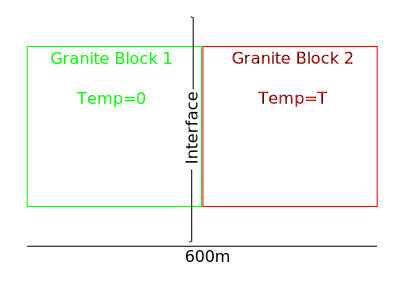
\includegraphics[width=4.in]{figures/onedheatdiff001}}
\caption{Example 1: Temperature differential along a single interface between
two granite blocks.}
\label{fig:onedgbmodel}
\end{figure}

\section{Example 1: One Dimensional Heat Diffusion in Granite}
\label{Sec:1DHDv00}

The first model consists of two blocks of isotropic material, for instance
granite, sitting next to each other.
Initial temperature in \textit{Block 1} is \verb|T1| and in \textit{Block 2} is
\verb|T2|.
We assume that the system is insulated.
What would happen to the temperature distribution in each block over time? 
Intuition tells us that heat will be transported from the hotter block to the
cooler one until both
blocks have the same temperature.

\subsection{1D Heat Diffusion Equation}
We can model the heat distribution of this problem over time using the one
dimensional heat diffusion equation\footnote{A detailed discussion on how the
heat diffusion equation is derived can be found at
\url{
http://online.redwoods.edu/instruct/darnold/DEProj/sp02/AbeRichards/paper.pdf}};
which is defined as:
\begin{equation}
\rho c\hackscore p \frac{\partial T}{\partial t} - \kappa \frac{\partial^{2}
T}{\partial x^{2}} = q\hackscore H 
\label{eqn:hd}
\end{equation}
where $\rho$ is the material density, $c\hackscore p$ is the specific heat and
$\kappa$ is the thermal 
conductivity\footnote{A list of some common thermal conductivities is available
from Wikipedia
\url{http://en.wikipedia.org/wiki/List_of_thermal_conductivities}}. Here we
assume that these material 
parameters are \textbf{constant}. 
The heat source is defined by the right hand side of \refEq{eqn:hd} as
$q\hackscore{H}$; this can take the form of a constant or a function of time and
space. For example $q\hackscore{H} = q\hackscore{0}e^{-\gamma t}$ where we have
the output of our heat source decaying with time. There are also two partial
derivatives in \refEq{eqn:hd}; $\frac{\partial T}{\partial t}$ describes the
change in temperature with time while $\frac{\partial ^2 T}{\partial x^2}$ is
the spatial change of temperature. As there is only a single spatial dimension
to our problem, our temperature solution $T$ is only dependent on the time $t$
and our signed distance from the block-block interface $x$.

\subsection{PDEs and the General Form}
It is possible to solve PDE \refEq{eqn:hd} analytically and obtain an exact
solution to our problem. However, it is not always practical to solve the
problem this way. Alternatively, computers can be used to find the solution. To
do this, a numerical approach is required to discretise 
the PDE \refEq{eqn:hd} across time and space, this reduces the problem to a
finite number of equations for a finite number of spatial points and time steps.
These parameters together define the model. While discretisation introduces
approximations and a degree of error, a sufficiently sampled model is generally
accurate enough to satisfy the accuracy requirements for the final solution.

Firstly, we discretise the PDE \refEq{eqn:hd} in time. This leaves us with a
steady linear PDE which involves spatial derivatives only and needs to be solved
in each time step to progress in time. \esc can help us here.

For time discretisation we use the Backward Euler approximation
scheme\footnote{see \url{http://en.wikipedia.org/wiki/Euler_method}}. It is
based on the approximation 
\begin{equation}
\frac{\partial T(t)}{\partial t} \approx \frac{T(t)-T(t-h)}{h}
\label{eqn:beuler}
\end{equation}
for  $\frac{\partial T}{\partial t}$  at time $t$ 
where $h$ is the time step size. This can also be written as;
\begin{equation}
\frac{\partial T}{\partial t}(t^{(n)}) \approx \frac{T^{(n)} - T^{(n-1)}}{h}
\label{eqn:Tbeuler}
\end{equation}
where the upper index $n$ denotes the n\textsuperscript{th} time step. So one
has
\begin{equation}
\begin{array}{rcl}
t^{(n)} & = & t^{(n-1)}+h \\
T^{(n)} & = & T(t^{(n-1)}) \\ 
\end{array}
\label{eqn:Neuler}
\end{equation}
Substituting \refEq{eqn:Tbeuler} into \refEq{eqn:hd} we get;
\begin{equation}
\frac{\rho c\hackscore p}{h} (T^{(n)} - T^{(n-1)}) - \kappa \frac{\partial^{2}
T^{(n)}}{\partial x^{2}} = q\hackscore H 
\label{eqn:hddisc}
\end{equation}
Notice that we evaluate the spatial derivative term at the current time
$t^{(n)}$ - therefore the name \textbf{backward Euler} scheme. Alternatively,
one can evaluate the spatial derivative term at the previous time $t^{(n-1)}$.
This approach is called the \textbf{forward Euler} scheme. This scheme can
provide some computational advantages, which
are not discussed here. However, the \textbf{forward Euler} scheme has a major
disadvantage. Namely, depending on the 
material parameters as well as the domain discretization of the spatial
derivative term, the time step size $h$ needs to be chosen sufficiently small to
achieve a stable temperature when progressing in time. Stability is achieved if
the temperature does not grow beyond its initial bounds and becomes
non-physical. 
The backward Euler scheme, which we use here, is unconditionally stable meaning
that under the assumption of a
physically correct problem set-up the temperature approximation remains physical
for all time steps. 
The user needs to keep in mind that the discretisation error introduced by
\refEq{eqn:beuler} 
is sufficiently small, thus a good approximation of the true temperature is
computed. It is therefore very important that any results are viewed with
caution. For example, one may compare the results for different time and
spatial step sizes.

To get the temperature $T^{(n)}$ at time $t^{(n)}$ we need to solve the linear 
differential equation \refEq{eqn:hddisc} which only includes spatial
derivatives. To solve this problem we want to use \esc. 

In \esc any given PDE can be described by the general form. For the purpose of
this introduction we illustrate a simpler version of the general form for full
linear PDEs which is available in the \esc user's guide. A simplified form that
suits our heat diffusion problem\footnote{The form in the \esc users guide which
uses the Einstein convention is written as 
$-(A\hackscore{jl} u\hackscore{,l})\hackscore{,j}+D u =Y$}
is described by;
\begin{equation}\label{eqn:commonform nabla}
-\nabla\cdot(A\cdot\nabla u) + Du = f
\end{equation}
where $A$, $D$ and $f$ are known values and $u$ is the unknown solution. The
symbol $\nabla$ which is called the \textit{Nabla operator} or \textit{del
operator} represents
the spatial derivative of its subject - in this case $u$. Lets assume for a
moment that we deal with a one-dimensional problem then ;
\begin{equation}
\nabla = \frac{\partial}{\partial x}
\end{equation}
and we can write \refEq{eqn:commonform nabla} as;
\begin{equation}\label{eqn:commonform}
-A\frac{\partial^{2}u}{\partial x^{2}} + Du = f
\end{equation}
if $A$ is constant. To match this simplified general form to our problem
\refEq{eqn:hddisc} 
we rearrange \refEq{eqn:hddisc};
\begin{equation}
\frac{\rho c\hackscore p}{h} T^{(n)} - \kappa \frac{\partial^2 T^{(n)}}{\partial
x^2} = q\hackscore H +  \frac{\rho c\hackscore p}{h} T^{(n-1)}
\label{eqn:hdgenf}
\end{equation}
The PDE is now in a form that satisfies \refEq{eqn:commonform nabla} which is
required for \esc to solve our PDE. This can be done by generating a solution
for successive increments in the time nodes $t^{(n)}$ where 
$t^{(0)}=0$ and  $t^{(n)}=t^{(n-1)}+h$ where $h>0$ is the step size and assumed
to be constant. 
In the following the upper index ${(n)}$ refers to a value at time $t^{(n)}$.
Finally, by comparing \refEq{eqn:hdgenf} with \refEq{eqn:commonform} one can see
that;
\begin{equation}\label{ESCRIPT SET}
u=T^{(n)}; 
A = \kappa; D = \frac{\rho c \hackscore{p}}{h}; f = q \hackscore{H} + \frac{\rho
c\hackscore p}{h} T^{(n-1)}
\end{equation}

\subsection{Boundary Conditions}
\label{SEC BOUNDARY COND}
With the PDE sufficiently modified, consideration must now be given to the
boundary conditions of our model. Typically there are two main types of boundary
conditions known as \textbf{Neumann} and \textbf{Dirichlet} boundary
conditions\footnote{More information on Boundary Conditions is available at
Wikipedia \url{http://en.wikipedia.org/wiki/Boundary_conditions}},
respectively. 
A \textbf{Dirichlet boundary condition} is conceptually simpler and is used to
prescribe a known value to the unknown solution (in our example the temperature)
on parts of the boundary or on the entire boundary of the region of interest. 
We discuss the Dirichlet boundary condition in our second example presented in
Section~\ref{Sec:1DHDv0}.

However, for this example we have made the model assumption that the system is
insulated, so we need to add an appropriate boundary condition to prevent
any loss or inflow of energy at the boundary of our domain. Mathematically this
is expressed by prescribing
the heat flux $\kappa \frac{\partial T}{\partial x}$  to zero. In our simplified
one dimensional model this is expressed
in the form;
\begin{equation}
\kappa \frac{\partial T}{\partial x}  = 0 
\end{equation}
or in a more general case as
\begin{equation}\label{NEUMAN 1}
\kappa \nabla T \cdot n  = 0 
\end{equation}
where $n$  is the outer normal field \index{outer normal field} at the surface
of the domain. 
The $\cdot$ (dot) refers to the dot product of the vectors $\nabla T$ and $n$.
In fact, the term $\nabla T \cdot n$ is the normal derivative of 
the temperature $T$. Other notations used here are\footnote{The \esc notation
for the normal
derivative is $T\hackscore{,i} n\hackscore i$.};
\begin{equation}
\nabla T \cdot n  = \frac{\partial T}{\partial n} \; .
\end{equation}
A condition of the type \refEq{NEUMAN 1} defines a \textbf{Neumann boundary
condition} for the PDE. 

The PDE \refEq{eqn:hdgenf} 
and the Neumann boundary condition~\ref{eqn:hdgenf} (potentially together with
the Dirichlet boundary conditions)  define a \textbf{boundary value problem}. 
It is the nature of a boundary value problem to allow making statements about
the solution in the
interior of the domain from information known on the boundary only. In most
cases we use the term partial differential equation but in fact it is a
boundary value problem. 
It is important to keep in mind that boundary conditions need to be complete and
consistent in the sense that 
at any point on the boundary either a Dirichlet or a Neumann boundary condition
must be set.

Conveniently, \esc makes a default assumption on the boundary conditions which
the user may modify where appropriate. 
For a problem of the form in~\refEq{eqn:commonform nabla} the default
condition\footnote{In the \esc user guide which uses the Einstein convention
this is written as 
$n\hackscore{j}A\hackscore{jl} u\hackscore{,l}=0$.} is;
\begin{equation}\label{NEUMAN 2}
-n\cdot A \cdot\nabla u = 0 
\end{equation}
which is used everywhere on the boundary. Again $n$ denotes the outer normal
field. 
Notice that the coefficient $A$ is the same as in the \esc
PDE~\ref{eqn:commonform nabla}. 
With the settings for the coefficients we have already identified in
\refEq{ESCRIPT SET} this
condition translates into 
\begin{equation}\label{NEUMAN 2b}
\kappa \frac{\partial T}{\partial x} = 0 
\end{equation}
for the boundary of the domain. This is identical to the Neumann boundary
condition we want to set. \esc will take care of this condition for us. We
discuss the Dirichlet boundary condition later.

\subsection{Outline of the Implementation}
\label{sec:outline}
To solve the heat diffusion equation (\refEq{eqn:hd}) we write a simple \pyt
script. At this point we assume that you have some basic understanding of the
\pyt programming language. If not, there are some pointers and links available
in Section \ref{sec:escpybas}. The script (discussed in \refSec{sec:key}) has
four major steps. Firstly, we need to define the domain where we want to 
calculate the temperature. For our problem this is the joint blocks of granite
which has a rectangular shape. Secondly, we need to define the PDE to solve in
each time step to get the updated temperature. Thirdly, we need to define the
coefficients of the PDE and finally we need to solve the PDE. The last two steps
need to be repeated until the final time marker has been reached. The work flow
is described in \reffig{fig:wf}.
% \begin{enumerate}
%  \item create domain
%  \item create PDE
%  \item while end time not reached:
% \begin{enumerate}
%  \item set PDE coefficients
%  \item solve PDE
%  \item update time marker
% \end{enumerate}
% \item end of calculation
% \end{enumerate}

\begin{figure}[h!]
 \centering
   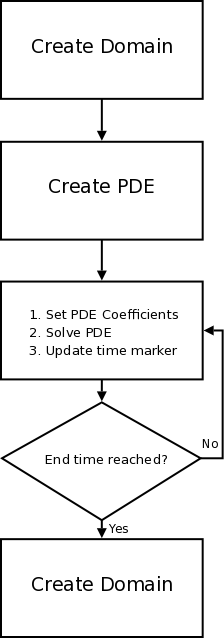
\includegraphics[width=1in]{figures/workflow.png}
   \caption{Workflow for developing an \esc model and solution}
   \label{fig:wf}
\end{figure}

In the terminology of \pyt, the domain and PDE are represented by
\textbf{objects}. The nice feature of an object is that it is defined by its
usage and features
rather than its actual representation. So we will create a domain object to
describe the geometry of the two
granite blocks. Then we define PDEs and spatially distributed values such as the
temperature 
on this domain. Similarly, to define a PDE object we use the fact that one needs
only to define the coefficients of the PDE and solve the PDE. The PDE object has
advanced features, but these are not required in simple cases.


\begin{figure}[t]
 \centering
   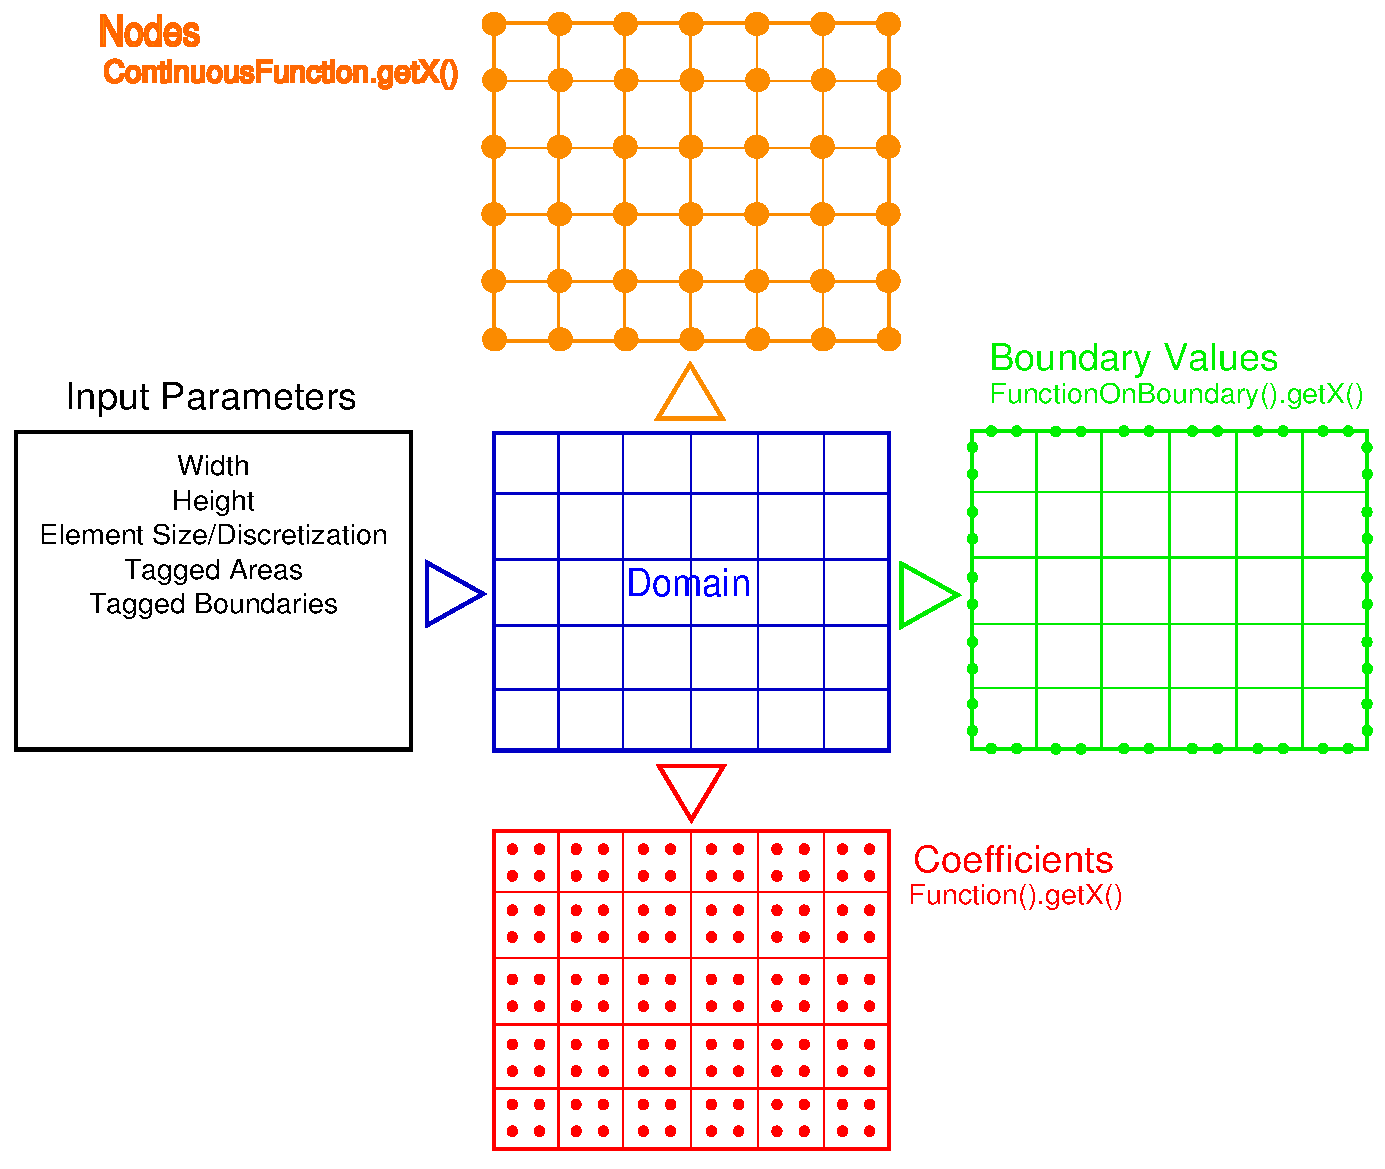
\includegraphics[width=6in]{figures/functionspace.pdf}
   \caption{\esc domain construction overview}
   \label{fig:fs}
\end{figure}

\subsection{The Domain Constructor in \esc}
\label{ss:domcon}
Whilst it is not strictly relevant or necessary, a better understanding of
how values are spatially distributed (\textit{e.g.} Temperature) and how PDE
coefficients are interpreted in \esc can be helpful.

There are various ways to construct domain objects. The simplest form is a
rectangular shaped region with a length and height. There is
a ready to use function for this named \verb rectangle(). Besides the spatial
dimensions this function requires to specify the number of
elements or cells to be used along the length and height, see \reffig{fig:fs}.
Any spatially distributed value 
and the PDE is represented in discrete form using this element
representation\footnote{We use the finite element method (FEM), see
\url{http://en.wikipedia.org/wiki/Finite_element_method} for details.}.
Therefore we will have access to an approximation of the true PDE solution
only. 
The quality of the approximation depends - besides other factors - mainly on the
number of elements being used. In fact, the 
approximation becomes better when more elements are used. However, computational
cost grows with the number of
elements being used. It is therefore important that you find the right balance
between the demand in accuracy and acceptable resource usage.

In general, one can think about a domain object as a composition of nodes and
elements. 
As shown in \reffig{fig:fs}, an element is defined by the nodes that are used to
describe its vertices. 
To represent spatially distributed values the user can use 
the values at the nodes, at the elements in the interior of the domain or at the
elements located on the surface of the domain. 
The different approach used to represent values is called \textbf{function
space} and is attached to all objects
in \esc representing a spatially distributed value such as the solution of
a PDE. The three function spaces we use at the moment are;
\begin{enumerate}
\item the nodes, called by \verb|ContinuousFunction(domain)| ;
\item the elements/cells, called by \verb|Function(domain)| ; and
\item the boundary, called by \verb|FunctionOnBoundary(domain)|.
\end{enumerate}
A function space object such as \verb|ContinuousFunction(domain)| has the method
\verb|getX| attached to it. This method returns the
location of the so-called \textbf{sample points} used to represent values of the
particular function space. So the
call \verb|ContinuousFunction(domain).getX()| will return the coordinates of the
nodes used to describe the domain while
\verb|Function(domain).getX()| returns the coordinates of numerical
integration points within elements, see \reffig{fig:fs}. 

This distinction between different representations of spatially distributed
values 
is important in order to be able to vary the degrees of smoothness in a PDE
problem. 
The coefficients of a PDE do not need to be continuous, thus this qualifies as a
\verb|Function()| type. 
On the other hand a temperature distribution must be continuous and needs to be
represented with a \verb|ContinuousFunction()| function space.
An influx may only be defined at the boundary and is therefore a
\verb|FunctionOnBoundary()| object.  
\esc allows certain transformations of the function spaces. A
\verb|ContinuousFunction()| can be transformed into a
\verb|FunctionOnBoundary()| or \verb|Function()|. On the other hand there is
not enough information in a \verb|FunctionOnBoundary()| to transform it to a
\verb|ContinuousFunction()|.
These transformations, which are called \textbf{interpolation} are invoked
automatically by \esc if needed.

Later in this introduction we discuss how
to define specific areas of geometry with different materials which are
represented by different material coefficients such as the
thermal conductivities $\kappa$. A very powerful technique to define these types
of PDE 
coefficients is tagging. Blocks of materials and boundaries can be named and
values can be defined on subregions based on their names.
This is a method for simplifying PDE coefficient and flux definitions. It makes
scripting much easier and we will discuss this technique in
Section~\ref{STEADY-STATE HEAT REFRACTION}.


\subsection{A Clarification for the 1D Case}
\label{SEC: 1D CLARIFICATION}
It is necessary for clarification that we revisit our general PDE from
\refeq{eqn:commonform nabla} for a two dimensional domain. \esc is inherently
designed to solve problems that are multi-dimensional and so
\refEq{eqn:commonform nabla} needs to be read as a higher dimensional problem.
In the case of two spatial dimensions the \textit{Nabla operator} has in fact
two components $\nabla = (\frac{\partial}{\partial x}, \frac{\partial}{\partial
y})$. Assuming the coefficient $A$ is constant, the \refEq{eqn:commonform nabla}
takes the following form;
\begin{equation}\label{eqn:commonform2D}
-A\hackscore{00}\frac{\partial^{2}u}{\partial x^{2}} 
-A\hackscore{01}\frac{\partial^{2}u}{\partial x\partial y} 
-A\hackscore{10}\frac{\partial^{2}u}{\partial y\partial x} 
-A\hackscore{11}\frac{\partial^{2}u}{\partial y^{2}} 
+ Du = f
\end{equation}
Notice that for the higher dimensional case $A$ becomes a matrix. It is also
important to notice that the usage of the Nabla operator creates
a compact formulation which is also independent from the spatial dimension. 
To make the general PDE \refEq{eqn:commonform2D} one dimensional as
shown in \refEq{eqn:commonform} we need to set
\begin{equation}
A\hackscore{00}=A; A\hackscore{01}=A\hackscore{10}=A\hackscore{11}=0
\end{equation}


\subsection{Developing a PDE Solution Script}
\label{sec:key}
\sslist{example01a.py}
We write a simple \pyt script which uses the \modescript, \modfinley and \modmpl
modules. 
By developing a script for \esc, the heat diffusion equation can be solved at
successive time steps for a predefined period using our general form
\refEq{eqn:hdgenf}. Firstly it is necessary to import all the
libraries\footnote{The libraries contain predefined scripts that are required to
solve certain problems, these can be simple like sine and cosine functions or
more complicated like those from our \esc library.} 
that we will require.
\begin{python}
from esys.escript import *
# This defines the LinearPDE module as LinearPDE
from esys.escript.linearPDEs import LinearPDE 
# This imports the rectangle domain function from finley.
from esys.finley import Rectangle 
# A useful unit handling package which will make sure all our units
# match up in the equations under SI.
from esys.escript.unitsSI import * 
\end{python}
It is generally a good idea to import all of the \modescript library, although
if the functions and classes required are known they can be specified
individually. The function \verb|LinearPDE| has been imported explicitly for
ease of use later in the script. \verb|Rectangle| is going to be our type of
domain. The module \verb|unitsSI| provides support for SI unit definitions with
our variables.

Once our library dependencies have been established, defining the problem
specific variables is the next step. In general the number of variables needed
will vary between problems. These variables belong to two categories. They are
either directly related to the PDE and can be used as inputs into the \esc
solver, or they are script variables used to control internal functions and
iterations in our problem. For this PDE there are a number of constants which
need values. Firstly, the domain upon which we wish to solve our problem needs
to be defined. There are different types of domains in \modescript which we
demonstrate in later tutorials but for our granite blocks, we simply use a
rectangular domain. 

Using a rectangular domain simplifies our granite blocks (which would in reality
be a \textit{3D} object) into a single dimension. The granite blocks will have a
lengthways cross section that looks like a rectangle.  As a result we do not
need to model the volume of the block due to symmetry. There are four arguments
we must consider when we decide to create a rectangular domain, the domain
\textit{length}, \textit{width} and \textit{step size} in each direction. When
defining the size of our problem it will help us determine appropriate values
for our model arguments. If we make our dimensions large but our step sizes very
small we increase the accuracy of our solution. Unfortunately we also increase
the number of calculations that must be solved per time step. This means more
computational time is required to produce a solution. In this \textit{1D}
problem, the bar is defined as being 1 metre long. An appropriate step size
\verb|ndx| would be 1 to 10\% of the length. Our \verb|ndy| needs only be 1,
this is because our problem stipulates no partial derivatives in the $y$
direction.
Thus the temperature does not vary with $y$. Hence, the model parameters can be
defined as follows; note we have used the \verb|unitsSI| convention to make sure
all our input units are converted to SI.
\begin{python}
mx = 500.*m #meters - model length
my = 100.*m #meters - model width
ndx = 50 # mesh steps in x direction 
ndy = 1 # mesh steps in y direction
boundloc = mx/2 # location of boundary between the two blocks
\end{python}
The material constants and the temperature variables must also be defined. For
the granite in the model they are defined as:
\begin{python}
#PDE related
rho = 2750. *kg/m**3 #kg/m^{3} density of iron
cp = 790.*J/(kg*K) # J/Kg.K thermal capacity
rhocp = rho*cp 
kappa = 2.2*W/m/K   # watts/m.Kthermal conductivity
qH=0 * J/(sec*m**3) # J/(sec.m^{3}) no heat source
T1=20 * Celsius # initial temperature at Block 1
T2=2273. * Celsius # base temperature at Block 2
\end{python}
Finally, to control our script we will have to specify our timing controls and
where we would like to save the output from the solver. This is simple enough:
\begin{python}
t=0 * day  #our start time, usually zero
tend=1. * day # - time to end simulation
outputs = 200 # number of time steps required.
h=(tend-t)/outputs #size of time step
#user warning statement
print "Expected Number of time outputs is: ", (tend-t)/h
i=0 #loop counter
\end{python}
Now that we know our inputs we will build a domain using the
\verb|Rectangle()| function from \FINLEY. The four arguments allow us to
define our domain \verb|model| as:
\begin{python}
#generate domain using rectangle
blocks = Rectangle(l0=mx,l1=my,n0=ndx, n1=ndy)
\end{python}
\verb|blocks| now describes a domain in the manner of Section \ref{ss:domcon}.

With a domain and all the required variables established, it is now possible to
set up our PDE so that it can be solved by \esc. The first step is to define the
type of PDE that we are trying to solve in each time step. In this example it is
a single linear PDE\footnote{in contrast to a system of PDEs which we discuss
later.}. We also need to state the values of our general form variables.
\begin{python}
mypde=LinearPDE(blocks)
A=zeros((2,2)))
A[0,0]=kappa
mypde.setValue(A=A, D=rhocp/h)
\end{python}
In many cases it may be possible to decrease the computational time of the
solver if the PDE is symmetric. 
Symmetry of a PDE is defined by;
\begin{equation}\label{eqn:symm}
A\hackscore{jl}=A\hackscore{lj}
\end{equation}
Symmetry is only dependent on the $A$ coefficient in the general form and the
other coefficients $D$ as well as the right hand side $Y$. From the above
definition we can see that our PDE is symmetric. The \verb|LinearPDE| class
provides the method \method{checkSymmetry} to check if the given PDE is
symmetric. As our PDE is symmetrical we enable symmetry via;
\begin{python}
myPDE.setSymmetryOn()
\end{python}
Next we need to establish the initial temperature distribution \verb|T|. We need
to 
assign the value \verb|T1| to all sample points left to the contact interface at
$x\hackscore{0}=\frac{mx}{2}$
and the value \verb|T2| right to the contact interface. \esc
provides the \verb|whereNegative| function to construct this. More
specifically, \verb|whereNegative| returns the value $1$ at those sample points
where the argument has a negative value. Otherwise zero is returned.
If \verb|x| are the $x\hackscore{0}$ 
coordinates of the sample points used to represent the temperature distribution 
then \verb|x[0]-boundloc| gives us a negative value for 
all sample points left to the interface and non-negative value to 
the right of the interface. So with;
\begin{python}
# ... set initial temperature ....
T= T1*whereNegative(x[0]-boundloc)+T2*(1-whereNegative(x[0]-boundloc))
\end{python}
we get the desired temperature distribution. To get the actual sample points
\verb|x| we use the \verb|getX()| method of the function space
\verb|Solution(blocks)| which is used to represent the solution of a PDE;
\begin{python}
x=Solution(blocks).getX()
\end{python}
As \verb|x| are the sample points for the function space
\verb|Solution(blocks)| 
the initial temperature \verb|T| is using these sample points for
representation.
Although \esc is trying to be forgiving with the choice of sample points and to
convert
where necessary the adjustment of the function space is not always possible. So
it is advisable to make a careful choice on the function space used.  

Finally we initialise an iteration loop to solve our PDE for all the time steps
we specified in the variable section. As the right hand side of the general form
is dependent on the previous values for temperature \verb T  across the bar this
must be updated in the loop. Our output at each time step is \verb T  the heat
distribution and \verb totT  the total heat in the system.
\begin{python}
while t < tend:
	i+=1 #increment the counter
	t+=h #increment the current time
	mypde.setValue(Y=qH+rhocp/h*T) # set variable PDE coefficients
	T=mypde.getSolution() #get the PDE solution
	totE = integrate(rhocp*T) #get the total heat (energy) in the system
\end{python}
The last statement in this script calculates the total energy in the system as
the volume integral of $\rho c\hackscore{p} T$ over the block.
As the blocks are insulated no energy should be lost or added. 
The total energy should stay constant for the example discussed here.

\subsection{Running the Script} 
The script presented so far is available under 
\verb|example01a.py|. You can edit this file with your favourite text editor. 
On most operating systems\footnote{The \texttt{run-escript} launcher is not
supported under {\it MS Windows} yet.} you can use the
\program{run-escript} command 
to launch {\it escript} scripts. For the example script use;
\begin{verbatim}
run-escript example01a.py
\end{verbatim}
The program will print a progress report. Alternatively, you can use 
the python interpreter directly;
\begin{verbatim}
python example01a.py
\end{verbatim}
if the system is configured correctly (please talk to your system
administrator).

\begin{figure}
\begin{center}
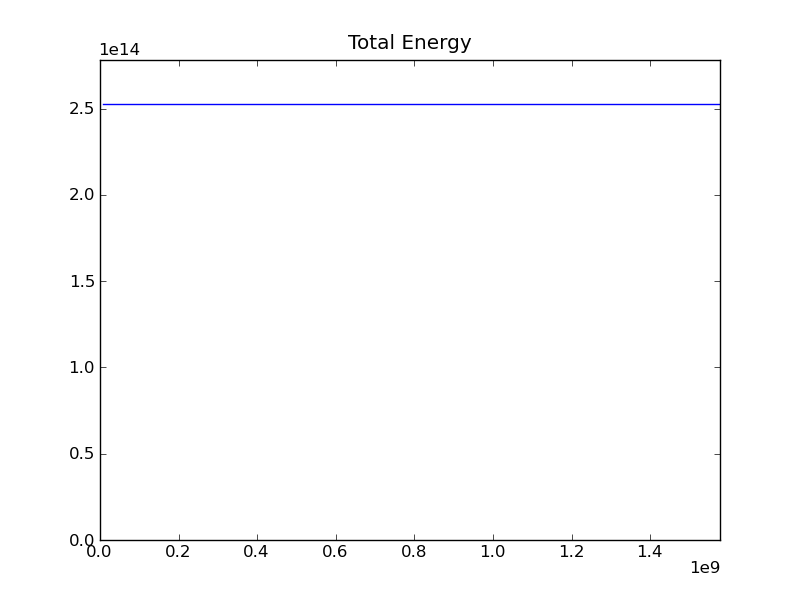
\includegraphics[width=4in]{figures/ttblockspyplot150}
\caption{Example 1b: Total Energy in the Blocks over Time (in seconds)}
\label{fig:onedheatout1} 
\end{center}
\end{figure}

\subsection{Plotting the Total Energy} 
\sslist{example01b.py}

\esc does not include its own plotting capabilities. However, it is possible to
use a variety of free \pyt packages for visualisation.
Two types will be demonstrated in this cookbook;
\mpl\footnote{\url{http://matplotlib.sourceforge.net/}} and 
\verb|VTK|\footnote{\url{http://www.vtk.org/}}. 
The \mpl package is a component of SciPy\footnote{\url{http://www.scipy.org}}
and is good for basic graphs and plots. 
For more complex visualisation tasks, in particular two and three dimensional
problems we recommend the use of more advanced tools. For instance,  \mayavi
\footnote{\url{http://code.enthought.com/projects/mayavi/}}
which is based upon the \verb|VTK| toolkit. The usage of \verb|VTK| based 
visualisation is discussed in Chapter~\ref{Sec:2DHD} which focuses on a two
dimensional PDE. 

For our simple granite block problem, we have two plotting tasks. Firstly, we
are interested in showing the
behaviour of the total energy over time and secondly, how the temperature
distribution within the block is developing over time.
Let us start with the first task.

The idea is to create a record of the time marks and the corresponding total
energies observed.
\pyt provides the concept of lists for this. Before 
the time loop is opened we create empty lists for the time marks \verb|t_list|
and the total energies \verb|E_list|. 
After the new temperature has been calculated by solving the PDE we append the
new time marker and the total energy value for that time
to the corresponding list using the \verb|append| method. With these
modifications our script looks as follows:
\begin{python}
t_list=[]
E_list=[]
# ... start iteration:
while t<tend:
      t+=h
      mypde.setValue(Y=qH+rhocp/h*T) # set variable PDE coefficients
      T=mypde.getSolution() #get the PDE solution
      totE=integrate(rhocp*T) 
      t_list.append(t)   # add current time mark to record
      E_list.append(totE) # add current total energy to record
\end{python}
To plot $t$ over $totE$ we use \mpl a module contained within \pylab which needs
to be loaded before use;
\begin{python}
import pylab as pl # plotting package.
\end{python}
Here we are not using \verb|from pylab import *| in order to avoid name
clashes for function names within \esc. 

The following statements are added to the script after the time loop has been
completed;
\begin{python}
pl.plot(t_list,E_list)
pl.title("Total Energy")
pl.axis([0,max(t_list),0,max(E_list)*1.1])
pl.savefig("totE.png")
\end{python}
The first statement hands over the time marks and corresponding total energies
to the plotter.
The second statement sets the title for the plot. The third statement
sets the axis ranges. In most cases these are set appropriately by the plotter.
 
The last statement generates the plot and writes the result into the file
\verb|totE.png| which can be displayed by (almost) any image viewer. 
As expected the total energy is constant over time, see
\reffig{fig:onedheatout1}.

\subsection{Plotting the Temperature Distribution}
\label{sec: plot T}
\sslist{example01c.py}
For plotting the spatial distribution of the temperature we need to modify the
strategy we have used for the total energy.
Instead of producing a final plot at the end we will generate a 
picture at each time step which can be browsed as a slide show or composed into
a movie.
The first problem we encounter is that if we produce an image at each time step
we need to make sure that the images previously generated are not overwritten.

To develop an incrementing file name we can use the following convention. It is
convenient to put all image files showing the same variable - in our case the
temperature distribution - into a separate directory.
As part of the \verb|os| module\footnote{The \texttt{os} module provides 
a powerful interface to interact with the operating system, see
\url{http://docs.python.org/library/os.html}.} \pyt 
provides the \verb|os.path.join| command to build file and directory names in a
platform independent way. Assuming that 
\verb|save_path| is the name of the directory we want to put the results in the
command is; 
\begin{python}
import os
os.path.join(save_path, "tempT%03d.png"%i )
\end{python}
where \verb|i| is the time step counter.
There are two arguments to the \verb|join| command. The \verb|save_path|
variable is a predefined string pointing to the directory we want to save our
data, for example a single sub-folder called \verb|data| would be defined by;
\begin{verbatim}
save_path = "data"
\end{verbatim}
while a sub-folder of \verb|data| called \verb|example01| would be defined by;
\begin{verbatim}
save_path = os.path.join("data","example01")
\end{verbatim}
The second argument of \verb|join| contains a string which is the file
name or subdirectory name. We can use the operator \verb|%| to use the value of
\verb|i| as part of our filename. The sub-string \verb|%03d| indicates that we
want to substitute a value into the name; 
\begin{itemize}
 \item \verb 0  means that small numbers should have leading zeroes;
 \item \verb 3  means that numbers should be written using at least 3 digits;
and
 \item \verb d  means that the value to substitute will be a decimal integer.
\end{itemize}
To actually substitute the value of \verb|i| into the name write \verb|%i| after
the string.
When done correctly, the output files from this command will be placed in the
directory defined by \verb save_path  as;
\begin{verbatim}
blockspyplot001.png
blockspyplot002.png
blockspyplot003.png
...
\end{verbatim}
and so on.

A sub-folder check/constructor is available in \esc. The command;
\begin{verbatim}
mkDir(save_path)
\end{verbatim}
will check for the existence of \verb save_path  and if missing, create the
required directories.

We start by modifying our solution script.
Prior to the \verb|while| loop we need to extract our finite solution
points to a data object that is compatible with \mpl. First we create the node
coordinates of the sample points used to represent
the temperature as a \pyt list of tuples or a \numpy array as requested by the
plotting function. 
We need to convert the array \verb|x| previously set as
\verb|Solution(blocks).getX()| into a \pyt list 
and then to a \numpy array. The $x\hackscore{0}$ component is then extracted via
an array slice to the variable \verb|plx|; 
\begin{python}
import numpy as np # array package.
#convert solution points for plotting
plx = x.toListOfTuples() 
plx = np.array(plx) # convert to tuple to numpy array
plx = plx[:,0] # extract x locations
\end{python}

\begin{figure}
\begin{center}
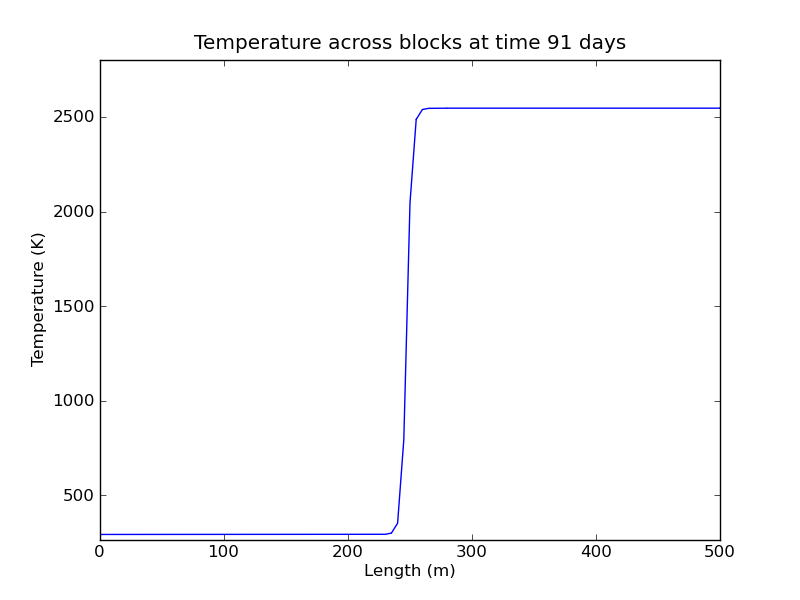
\includegraphics[width=4in]{figures/blockspyplot001}
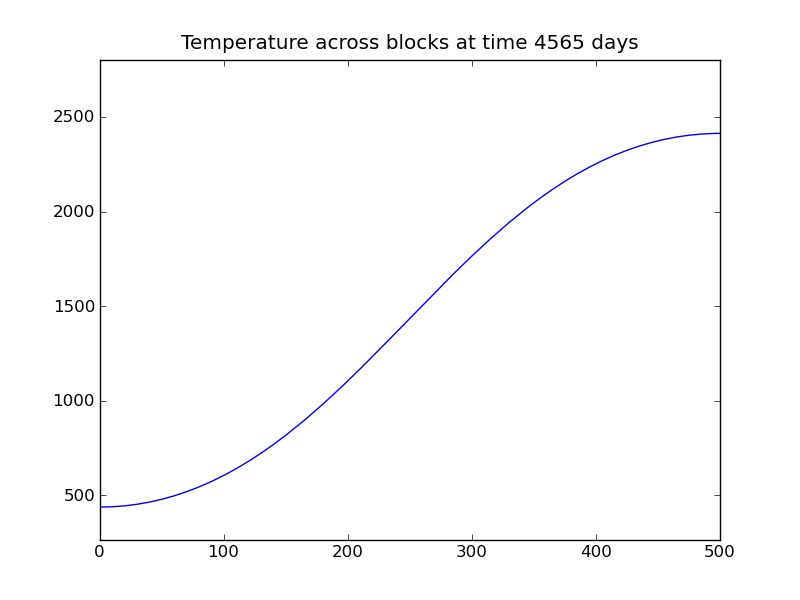
\includegraphics[width=4in]{figures/blockspyplot050}
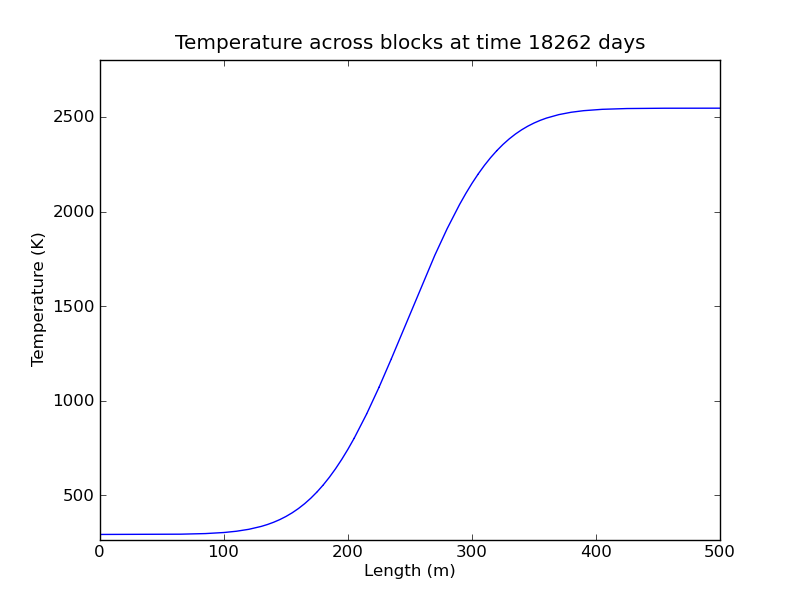
\includegraphics[width=4in]{figures/blockspyplot200}
\caption{Example 1c: Temperature ($T$) distribution in the blocks at time steps
$1$, $50$ and $200$}
\label{fig:onedheatout} 
\end{center}
\end{figure}

We use the same techniques provided by \mpl as we have used to plot the total
energy over time. 
For each time step we generate a plot of the temperature distribution and save
each to a file. 
The following is appended to the end of the \verb|while| loop and creates one
figure of the temperature distribution. We start by converting the solution to a
tuple and then plotting this against our \textit{x coordinates} \verb|plx| we
have generated before. We add a title to the diagram before it is rendered into
a file. 
Finally, the figure is saved to a \verb|*.png| file and cleared for the
following iteration.
\begin{python}
# ... start iteration:
while t<tend:
        ....
	T=mypde.getSolution() #get the PDE solution
        tempT = T.toListOfTuples() # convert to a tuple
        pl.plot(plx,tempT) # plot solution
	# set scale (Temperature should be between Tref and T0)
        pl.axis([0,mx,Tref*.9,T0*1.1])
        # add title
	pl.title("Temperature across the blocks at time %e minutes"%(t/day))
	#save figure to file
	pl.savefig(os.path.join(save_path,"tempT","blockspyplot%03d.png") %i)
\end{python}
Some results are shown in \reffig{fig:onedheatout}. 

\subsection{Making a Video} 
Our saved plots from the previous section can be cast into a video using the
following command appended to the end of the script. The \verb mencoder command
is not available on every platform, so some users need to use an alternative
video encoder.
\begin{python}
# compile the *.png files to create a *.avi video that shows T change
# with time. This operation uses Linux mencoder. For other operating 
# systems it is possible to use your favourite video compiler to
# convert image files to videos.

os.system("mencoder mf://"+save_path+"/tempT"+"/*.png -mf type=png:\
           w=800:h=600:fps=25 -ovc lavc -lavcopts vcodec=mpeg4 -oac copy -o \
           example01tempT.avi")
\end{python}
 


%%%%%%%%%%%%%%%%%%%%%%%%%%%%%%%%%%%%%%%%%%%%%%%%%%%%%%%%
%
% Copyright (c) 2003-2010 by University of Queensland
% Earth Systems Science Computational Center (ESSCC)
% http://www.uq.edu.au/esscc
%
% Primary Business: Queensland, Australia
% Licensed under the Open Software License version 3.0
% http://www.opensource.org/licenses/osl-3.0.php
%
%%%%%%%%%%%%%%%%%%%%%%%%%%%%%%%%%%%%%%%%%%%%%%%%%%%%%%%%
\begin{figure}[ht]
\centerline{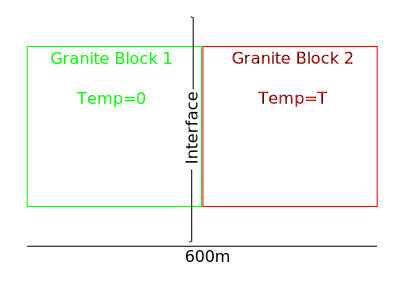
\includegraphics[width=4.in]{figures/onedheatdiff002}}
\caption{Example 2: One dimensional model of an Iron bar.}
\label{fig:onedhdmodel}
\end{figure}

\section{Example 2: One Dimensional Heat Diffusion in an Iron Rod}
\sslist{example02.py}
\label{Sec:1DHDv0}

Our second example is a cold iron bar at a constant temperature of $T\hackscore{ref}=20^{\circ} C$, see \reffig{fig:onedhdmodel}. The bar is perfectly insulated on all sides with a heating element at one end keeping the the temperature at a constant level $T\hackscore0=100^{\circ} C$.  As heat is applied; energy will disperse along the bar via conduction. With time the bar will reach a constant temperature equivalent to that of the heat source.

This problem is very similar to the example of temperature diffusion in granite blocks presented in the previous section~\ref{Sec:1DHDv00}. So we modify the script we have already developed for the granite blocks to adjust 
it to the iron bar problem.  
The obvious difference between the two problems are the dimensions of the domain and different materials involved. This will change the time scale of the model from years to hours. 
The new settings are;
\begin{python}
#Domain related.
mx = 1*m #meters - model length
my = .1*m #meters - model width
ndx = 100 # mesh steps in x direction 
ndy = 1 # mesh steps in y direction - one dimension means one element
#PDE related
rho = 7874. *kg/m**3 #kg/m^{3} density of iron
cp = 449.*J/(kg*K) # J/Kg.K thermal capacity
rhocp = rho*cp 
kappa = 80.*W/m/K   # watts/m.Kthermal conductivity
qH = 0 * J/(sec*m**3) # J/(sec.m^{3}) no heat source
Tref = 20 * Celsius  # base temperature of the rod
T0 = 100 * Celsius # temperature at heating element
tend= 0.5 * day # - time to end simulation
\end{python}
We also need to alter the initial value for the temperature. Now we need to set the 
temperature to $T\hackscore{0}$ at the left end of the rod where we have $x\hackscore{0}=0$ and 
$T\hackscore{ref}$ elsewhere. Instead of \verb|whereNegative| function we use now the 
\verb|whereZero| which returns the value one for those sample points where 
the argument (almost) equals zero and the value zero elsewhere. The initial
temperature is set to;
\begin{python}
# ... set initial temperature ....
T= T0*whereZero(x[0])+Tref*(1-whereZero(x[0]))
\end{python}

\subsection{Dirichlet Boundary Conditions}
In iron rod model  we want to keep the initial temperature $T\hackscore0$ on the left side of the domain over time. 
So when we solve the PDE~\refEq{eqn:hddisc} the solution must have the value $T\hackscore0$ on the left hand
side of the domain. As mentioned already in Section~\ref{SEC BOUNDARY COND} where we discussed
boundary condition this kind of condition are called a \textbf{Dirichlet boundary condition}. Some people also
use the term \textbf{constraint} for the PDE. 

To define a Dirichlet boundary condition we need to define where to apply the condition and what value the 
solution should have at these locations. In \esc we use $q$ and $r$ to define the Dirichlet boundary conditions
for a PDE. The solution $u$ of the PDE is set to $r$ for all sample points where $q$ has a positive value.
Mathematically this is expressed in the form;
\begin{equation}
  u(x) = r(x) \mbox{ for any } x \mbox{ with } q(x) > 0
\end{equation} 
In the case of the iron rod 
we can set;
\begin{python}
q=whereZero(x[0])
r=T0
\end{python}
to prescribe the value $T0$ for the temperature at the left end of the rod where $x\hackscore{0}=0$. 
Here we use the \verb|whereZero| function again which we have already used to set the initial value.
Notice that $r$ is set to the constant value $r$ for all sample points. In fact, 
values of $r$ are used only where $q$ is positive. Where $q$ is non-positive,
$r$ may have any value as these values are not used by the PDE solver. 

To set the Dirichlet boundary conditions for the PDE to be solved in each time step we need
to add some statements;
\begin{python}
mypde=LinearPDE(rod)
A=zeros((2,2)))
A[0,0]=kappa
q=whereZero(x[0])
mypde.setValue(A=A, D=rhocp/h, q=q, r=T0)
\end{python}
It is important to remark here that the Dirichlet condition \textbf{overwrites} any Neuman boundary 
condition \esc sets by default (or you may set).  

\begin{figure}
\begin{center}
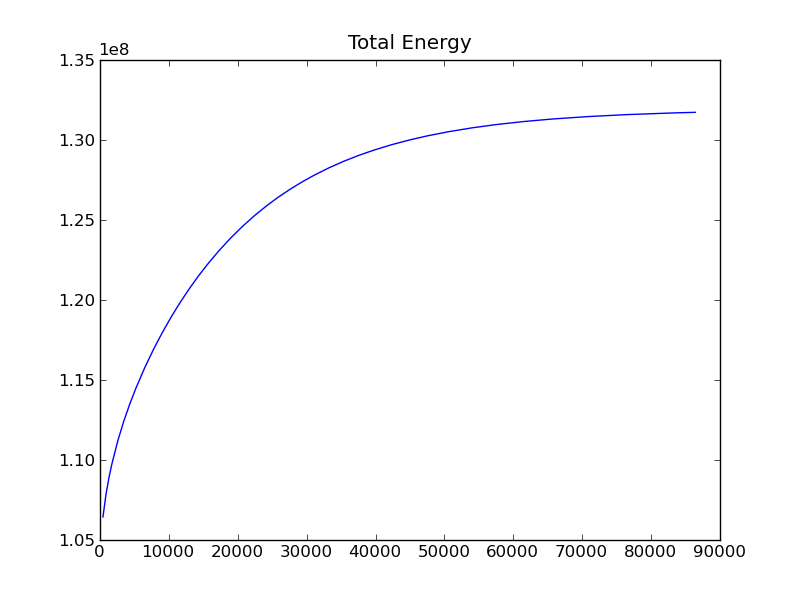
\includegraphics[width=4in]{figures/ttrodpyplot150}
\caption{Example 2: Total Energy in the Iron Rod over Time (in seconds).}
\label{fig:onedheatout1 002} 
\end{center}
\end{figure}

\begin{figure}
\begin{center}
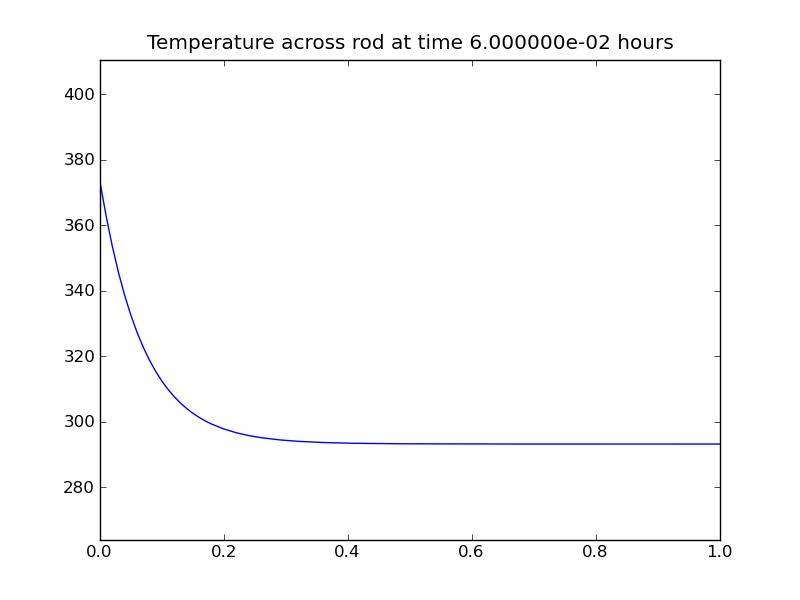
\includegraphics[width=4in]{figures/rodpyplot001}
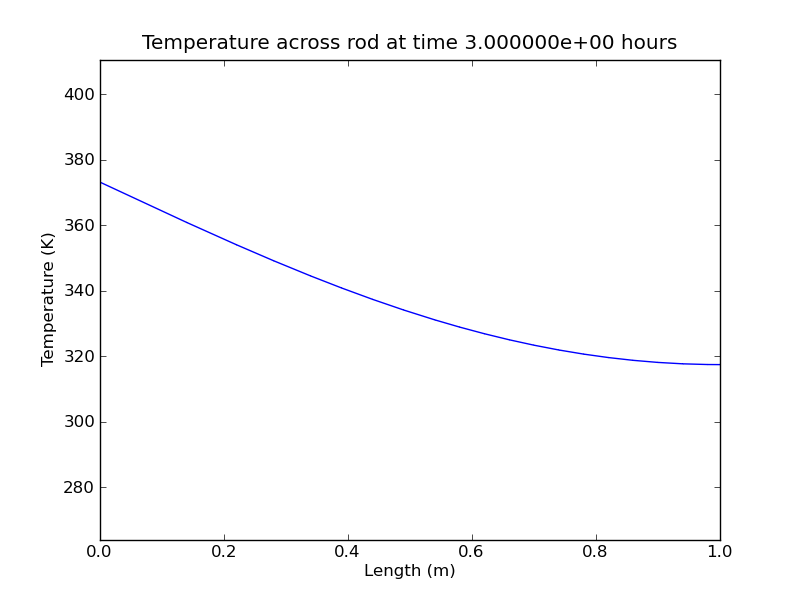
\includegraphics[width=4in]{figures/rodpyplot050}
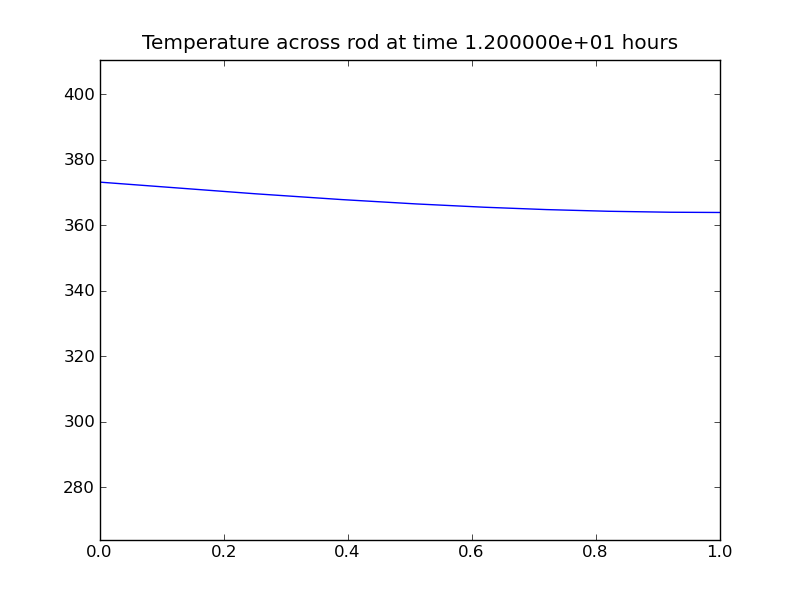
\includegraphics[width=4in]{figures/rodpyplot200}
\caption{Example 2: Temperature ($T$) distribution in the iron rod at time steps $1$, $50$ and $200$.}
\label{fig:onedheatout 002} 
\end{center}
\end{figure}

Besides some cosmetic modification this all we need to change. The total energy over time is shown in \reffig{fig:onedheatout1 002}. As heat
is transfered into the rod by the heater the total energy is growing over time but reaches a plateau 
when the temperature is constant is the rod, see \reffig{fig:onedheatout 002}. 
You will notice that the time scale of this model is several order of magnitudes faster than
for the granite rock problem due to the different length scale and material parameters. 
In practice it can take a few models run before the right time scale has been chosen\footnote{An estimate of the
time scale for a diffusion problem is given by the formula $\frac{\rho c\hackscore{p} L\hackscore{0}^2}{4 \kappa}$, see
\url{http://en.wikipedia.org/wiki/Fick\%27s_laws_of_diffusion}}.






\section{For the Reader}
\begin{enumerate}
 \item Move the boundary line between the two granite blocks to another part of the domain.
 \item Split the domain into multiple granite blocks with varying temperatures.
 \item Vary the mesh step size. Do you see a difference in the answers? What does happen with the compute time?
 \item Insert an internal heat source (Hint: The internal heat source is given by $q\hackscore{H}$.)
 \item Change the boundary condition for iron rod example such that the temperature 
 at the right end is kept at a constant level $T\hackscore{ref}$, which corresponds to the installation of a cooling element (Hint: Modify $q$ and $r$). 
\end{enumerate}



\chapter{The Second Dimension}
\label{CHAP HEAT 2a}

%%%%%%%%%%%%%%%%%%%%%%%%%%%%%%%%%%%%%%%%%%%%%%%%%%%%%%%%
%
% Copyright (c) 2003-2011 by University of Queensland
% Earth Systems Science Computational Center (ESSCC)
% http://www.uq.edu.au/esscc
%
% Primary Business: Queensland, Australia
% Licensed under the Open Software License version 3.0
% http://www.opensource.org/licenses/osl-3.0.php
%
%%%%%%%%%%%%%%%%%%%%%%%%%%%%%%%%%%%%%%%%%%%%%%%%%%%%%%%%

\begin{figure}[t]
\centerline{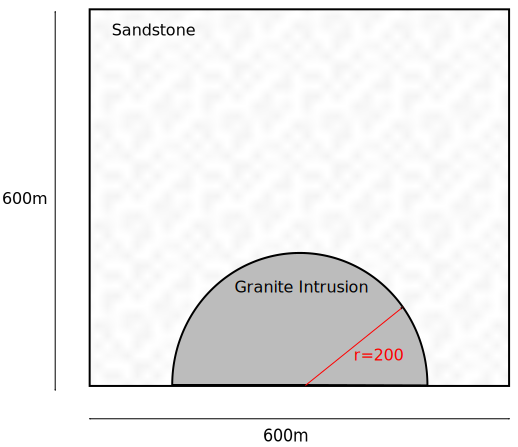
\includegraphics[width=4.in]{figures/twodheatdiff}}
\caption{Example 3: 2D model: granitic intrusion of sandstone country rock}
\label{fig:twodhdmodel}
\end{figure}

\sslist{example03a.py and cblib.py}

Building upon our success from the 1D models, it is now prudent to expand our
domain by another dimension. 
For this example we use a very simple magmatic intrusion as the basis for our
model. The simulation will be a single event where some molten granite has
formed a cylindrical dome at the base of some cold sandstone country rock.
Assuming that the cylinder is very long
we model a cross-section as shown in \reffig{fig:twodhdmodel}. We will implement
the same 
diffusion model as we have used for the granite blocks in \refSec{Sec:1DHDv00}
but will add the second spatial dimension and show how to define 
variables depending on the location of the domain. 
We use \file{onedheatdiff001b.py} as the starting point to develop this model. 

\section{Example 3: Two Dimensional Heat Diffusion for a basic Magmatic
Intrusion}
\label{Sec:2DHD}

To expand upon our 1D problem, the domain must first be expanded. In fact, we
have solved a two dimensional problem already but essentially ignored the second
dimension. In our definition phase we create a square domain in $x$ and
$y$\footnote{In \esc the notation
$x_{0}$ and $x_{1}$ is used for $x$ and $y$, respectively.}
that is $600$ meters along each side \reffig{fig:twodhdmodel}. Now we set the
number of discrete spatial cells to $150$ in both directions and the radius of
the intrusion to $200$ meters with the centre located at the $300$ meter mark
on the $x$-axis. Thus, the domain variables are;
\begin{python}
mx = 600*m #meters - model length
my = 600*m #meters - model width
ndx = 150 #mesh steps in x direction 
ndy = 150 #mesh steps in y direction
r = 200*m #meters - radius of intrusion
ic = [300*m, 0] #coordinates of the centre of intrusion (meters)
qH=0.*J/(sec*m**3) #our heat source temperature is zero
\end{python}
As before we use 
\begin{python}
model = Rectangle(l0=mx,l1=my,n0=ndx, n1=ndy)
\end{python}
to generate the domain. 

There are two fundamental changes to the PDE that we have discussed in
\refSec{Sec:1DHDv00}. Firstly,
because the material coefficients for granite and sandstone are different, we
need to deal with 
PDE coefficients which vary with their location in the domain. Secondly, we
need to deal with the second spatial dimension. We can investigate these two
modifications at the same time. 
In fact, the temperature model \refEq{eqn:hd} we utilised in
\refSec{Sec:1DHDv00} applied for the 
1D case with a constant material parameter only. For the more general case
examined in this chapter, the correct model equation is 
\begin{equation}
\rho c_p \frac{\partial T}{\partial t} -  \frac{\partial }{\partial x}
\kappa \frac{\partial T}{\partial x} -  \frac{\partial }{\partial y} \kappa
\frac{\partial T}{\partial y} = q_H 
\label{eqn:hd2}
\end{equation}
Notice that for the 1D case we have $\frac{\partial T}{\partial y}=0$ and
for the case of constant material parameters $\frac{\partial }{\partial x}
\kappa = \kappa  \frac{\partial }{\partial x}$ thus this new equation coincides
with a simplified model equation for this case. It is more convenient 
to write this equation using the $\nabla$ notation as we have already seen in
\refEq{eqn:commonform nabla};
\begin{equation}\label{eqn:Tform nabla}
\rho c_p \frac{\partial T}{\partial t} 
-\nabla \cdot \kappa \nabla T = q_H
\end{equation}
We can easily apply the backward Euler scheme as before to end up with 
\begin{equation}
\frac{\rho c_p}{h} T^{(n)} -\nabla \cdot \kappa \nabla T^{(n)}  =
q_H +  \frac{\rho c_p}{h} T^{(n-1)}
\label{eqn:hdgenf2}
\end{equation}
which is very similar to \refEq{eqn:hdgenf} used to define the temperature
update in the simple 1D case. 
The difference is in the second order derivative term
$\nabla \cdot \kappa \nabla T^{(n)}$. Under the light of the more general case
we need to revisit the \esc PDE form as shown in \ref{eqn:commonform2D}.
For the 2D case with variable PDE coefficients the form needs to be read as 
\begin{equation}\label{eqn:commonform2D 2}
-\frac{\partial }{\partial x} A_{00}\frac{\partial u}{\partial x} 
-\frac{\partial }{\partial x} A_{01}\frac{\partial u}{\partial y} 
-\frac{\partial }{\partial y} A_{10}\frac{\partial u}{\partial x} 
-\frac{\partial }{\partial x} A_{11}\frac{\partial u}{\partial y} 
+ Du = f
\end{equation}
So besides the settings $u=T^{(n)}$, $D = \frac{\rho c _{p}}{h}$ and
$f = q _{H} + \frac{\rho c_p}{h} T^{(n-1)}$ as we have used
before (see \refEq{ESCRIPT SET}) we need to set
\begin{equation}\label{eqn: kappa general}
A_{00}=A_{11}=\kappa; A_{01}=A_{10}=0
\end{equation}
The fundamental difference to the 1D case is that $A_{11}$ is not set
to zero but $\kappa$,
which brings in the second dimension. It is important to note that the
coefficients of the PDE may depend on their location in the domain which does
not influence the usage of the PDE form. This is very convenient as we can
introduce spatial dependence to the PDE coefficients without modification to
the way we call the PDE solver. 

A very convenient way to define the matrix $A$ in \refEq{eqn: kappa general}
can be carried out using the Kronecker $\delta$ symbol\footnote{see
\url{http://en.wikipedia.org/wiki/Kronecker_delta}}. The 
\esc function \verb|kronecker| returns this matrix;
\begin{equation}
\verb|kronecker(model)| = \left[ 
\begin{array}{cc}
 1 & 0 \\
 0 & 1 \\
\end{array}
\right]
\end{equation}
As the argument \verb|model| represents a two dimensional domain the matrix is
returned as a $2 \times 2$ matrix
(in the case of a three-dimensional domain a $3 \times 3$ matrix is returned).
The call 
\begin{python}
mypde.setValue(A=kappa*kronecker(model),D=rhocp/h)
\end{python}
sets the PDE coefficients according to \refEq{eqn: kappa general}.  

We need to check the boundary conditions before we turn to the question: how do
we set $\kappa$. As pointed out \refEq{NEUMAN 2} makes certain assumptions on
the boundary conditions. In our case these assumptions translate to;
\begin{equation}
-n \cdot \kappa \nabla T^{(n)} = 
-n_{0} \cdot \kappa \frac{\partial T^{(n)}}{\partial x} -
n_{1} \cdot  \kappa \frac{\partial T^{(n)}}{\partial y} = 0
\label{eq:hom flux}
\end{equation}
which sets the normal component of the heat flux $- \kappa \cdot (\frac{\partial
T^{(n)}}{\partial x}, \frac{\partial T^{(n)}}{\partial y})$ to zero. This means
that the region is insulated which is what we want. 
On the left and right face of the domain where we have
$(n_{0},n_{1} ) = (\mp 1,0)$ 
this means $\frac{\partial T^{(n)}}{\partial x}=0$ and on the top and bottom on
the domain 
where we have  $(n_{0},n_{1} ) = (\pm 1,0)$ this is
$\frac{\partial T^{(n)}}{\partial y}=0$. 

\section{Setting variable PDE Coefficients}
Now we need to look into the problem of how we define the material coefficients
$\kappa$ and $\rho c_p$ depending on their location in the domain. 
We can make use of the technique used in the granite block example in
\refSec{Sec:1DHDv00}
to set up the initial temperature. However,
the situation is more complicated here as we have to deal with a
curved interface between the two sub-domains.

Prior to setting up the PDE, the interface between the two materials must be
established. 
The distance $s\ge 0$ between two points $[x,y]$ and
$[x_{0},y_{0}]$ in Cartesian coordinates is defined as:
\begin{equation}
 (x-x_{0})^{2}+(y-y_{0})^{2} = s^{2}
\end{equation}
If we define the point $[x_{0},y_{0}]$ as $ic$ which denotes
the centre of the semi-circle of our intrusion, then for all the points $[x,y]$
in our model we can calculate a distance to $ic$. 
All the points that fall within the given radius $r$ of our intrusion will have
a corresponding 
value $s < r$ and all those belonging to the country rock will have a value $s >
r$. By subtracting $r$ from both of these conditions we find $s-r < 0$ for all
intrusion points and $s-r > 0$ for all country rock points. 
Defining these conditions within the script is quite simple and is done using
the following command:
\begin{python}
bound = length(x-ic)-r #where the boundary will be located
\end{python}
This definition of the boundary can now be used with the \verb|whereNegative|
command again to help define the material constants and temperatures in our
domain. 
If \verb|kappai| and \verb|kappac| are the 
thermal conductivities for the intrusion material granite and for the
surrounding sandstone, then we set; 
\begin{python}
x=Function(model).getX()
bound = length(x-ic)-r
kappa = kappai * whereNegative(bound) + kappac * (1-whereNegative(bound))
mypde.setValue(A=kappa*kronecker(model))
\end{python}
Notice that we are using the sample points of the \verb|Function| function space
as expected for the PDE coefficient \verb|A|\footnote{For the experienced user: use
\texttt{x=mypde.getFunctionSpace("A").getX()}.}.
The corresponding statements are used to set $\rho c_p$. 

Our PDE has now been properly established. The initial conditions for
temperature are set out in a similar manner:
\begin{python}
#defining the initial temperatures.
x=Solution(model).getX()
bound = length(x-ic)-r
T= Ti*whereNegative(bound)+Tc*(1-whereNegative(bound))
\end{python}
where \verb|Ti| and \verb|Tc| are the initial temperature in the regions of the
granite and surrounding sandstone, respectively. It is important to
notice that we reset \verb|x| and \verb|bound| to refer to the appropriate 
sample points of a PDE solution\footnote{For the experienced user: use
\texttt{x=mypde.getFunctionSpace("r").getX()}.}.

\begin{figure}[ht]
\centerline{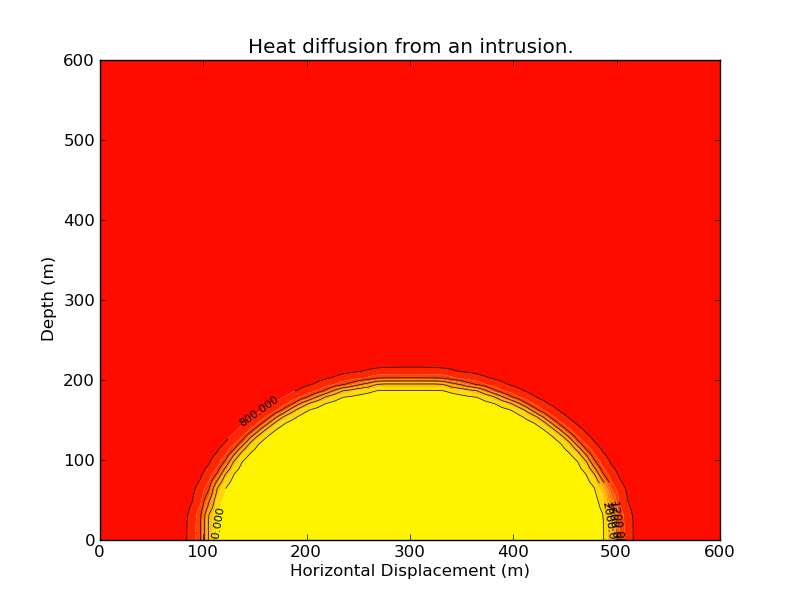
\includegraphics[width=4.in]{figures/heatrefraction001.png}}
\centerline{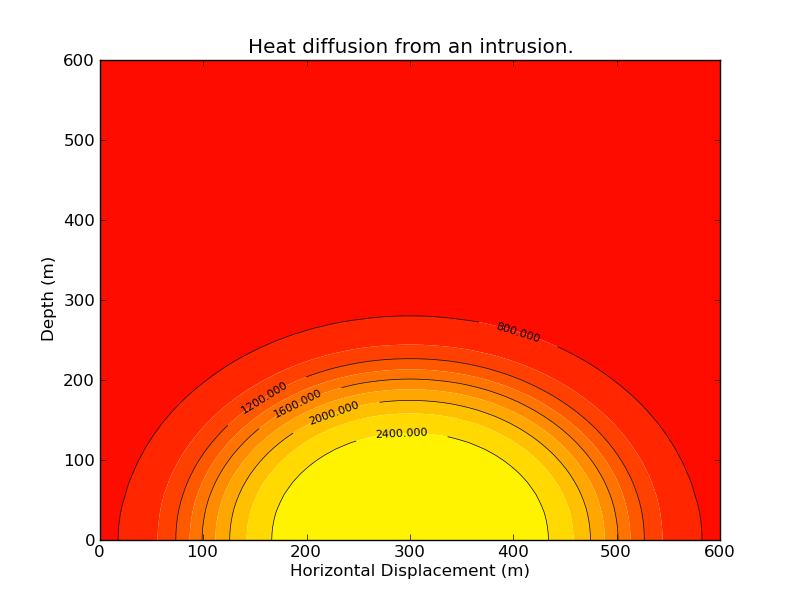
\includegraphics[width=4.in]{figures/heatrefraction030.png}}
\centerline{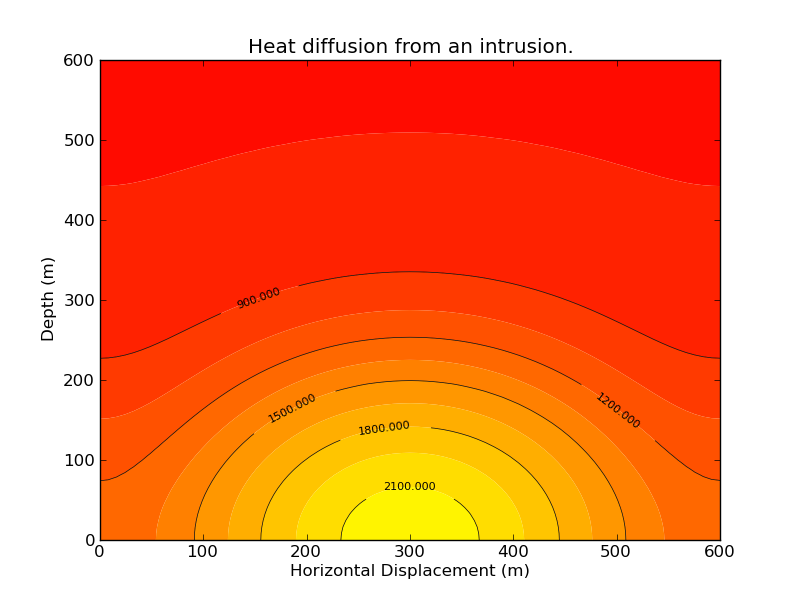
\includegraphics[width=4.in]{figures/heatrefraction200.png}}
\caption{Example 3a: 2D model: Total temperature distribution ($T$) at time step
$1$, $20$ and $200$. Contour lines show temperature.}
\label{fig:twodhdans}
\end{figure}

\section{Contouring \esc Data using \modmpl.}
\label{Sec:2DHD plot}
To complete our transition from a 1D to a 2D model we also need to modify the 
plotting procedure. As before we use \modmpl to do the plotting in this case a
contour plot. For 2D contour plots \modmpl expects that the data are regularly
gridded. We have no control over the location and ordering of the sample points
used to represent the solution. Therefore it is necessary to interpolate our
solution onto a regular grid.

In \refSec{sec: plot T} we have already learned how to extract the $x$
coordinates of sample points as 
\verb|numpy| array to hand the values to \modmpl. This can easily be extended
to extract both the $x$ and the $y$ coordinates;
\begin{python}
import numpy as np
def toXYTuple(coords):
    coords = np.array(coords.toListOfTuples()) #convert to Tuple
    coordX = coords[:,0] #X components.
    coordY = coords[:,1] #Y components.
    return coordX,coordY
\end{python}
For convenience we have put this function into \file{clib.py} so we can use
this function in other scripts more easily. 

We now generate a regular $100 \times 100$ grid over the domain ($mx$ and $my$ 
are the dimensions in the $x$ and $y$ directions) which is done using the
\modnumpy function \verb|linspace|.
\begin{python}
from clib import toXYTuple
# get sample points for temperature as  for contouring      
coordX, coordY = toXYTuple(T.getFunctionSpace().getX())
# create regular grid
xi = np.linspace(0.0,mx,75)
yi = np.linspace(0.0,my,75)
\end{python}
The values \verb|[xi[k], yi[l]]| are the grid points.

The remainder of our contouring commands resides within a \verb|while| loop so
that a new contour is generated for each time step. For each time step the
solution must be re-gridded for \modmpl using the \verb|griddata| function. This
function interprets irregularly located values \verb|tempT| at locations defined
by \verb|coordX| and \verb|coordY| as values at the new coordinates of a
rectangular grid defined by
\verb|xi| and \verb|yi|. The output is \verb|zi|. It is now possible to use the
\verb|contourf| function which generates colour filled contours. The colour
gradient of our plots is set via the command 
\verb|pl.matplotlib.pyplot.autumn()|, other colours are listed on the \modmpl web page\footnote{see
\url{http://matplotlib.sourceforge.net/api/}}. Our results are then contoured,
visually adjusted using the \modmpl functions and then saved to a file.
\verb|pl.clf()| clears the figure in readiness for the next time iteration.
\begin{python}
#grid the data.
zi = pl.matplotlib.mlab.griddata(coordX,coordY,tempT,xi,yi)
# contour the gridded data, plotting dots at the randomly spaced data points.
pl.matplotlib.pyplot.autumn()
pl.contourf(xi,yi,zi,10)
CS = pl.contour(xi,yi,zi,5,linewidths=0.5,colors='k')
pl.clabel(CS, inline=1, fontsize=8)
pl.axis([0,600,0,600])
pl.title("Heat diffusion from an intrusion.")
pl.xlabel("Horizontal Displacement (m)")
pl.ylabel("Depth (m)")
pl.savefig(os.path.join(save_path,"Tcontour%03d.png") %i)
pl.clf()        
\end{python}
The function \verb|pl.contour| is used to add labelled contour lines to the
plot. 
The results for selected time steps are shown in \reffig{fig:twodhdans}.


\section{Advanced Visualisation using VTK}

\sslist{example03b.py}
An alternative approach to \modmpl for visualisation is the usage of a package
which is based on the Visualization Toolkit (VTK) library\footnote{see \url{http://www.vtk.org/}}.
There is a variety of packages available. Here we use the package \mayavi\footnote{see
\url{http://code.enthought.com/projects/mayavi/}} as an example. 

\mayavi is an interactive, GUI driven tool which is 
really designed to visualise large three dimensional data sets where \modmpl 
is not suitable. But it is also very useful when it comes to two dimensional
problems. 
The decision of which tool is the best can be subjective and users should
determine which package they require and are most comfortable with. The main
difference between using \mayavi (or other VTK based tools) and \modmpl is that
the actual visualisation is detached from the calculation by writing the
results to external files and importing them into \mayavi. In 3D the best
camera position for rendering a scene is not obvious before the results are
available. Therefore the user may need to try different settings before the
best is found. Moreover, in many cases a 3D interactive visualisation is the
only way to really understand the results (e.g. using stereographic projection).

To write the temperatures at each time step to data files in the VTK file format
one needs to import \verb|saveVTK| from the \weipa module and call it:
\begin{python}
from esys.weipa import saveVTK
while t<=tend:
      i+=1 #counter
      t+=h #current time
      mypde.setValue(Y=qH+T*rhocp/h)
      T=mypde.getSolution()
      saveVTK(os.path.join(save_path,"data.%03d.vtu"%i, T=T)
\end{python}
The data files, e.g. \file{data.001.vtu}, contain all necessary information to 
visualise the temperature and can be directly processed by \mayavi. Note that
there is no re-gridding required. The file extension \file{.vtu} is
automatically added if not supplied to \verb|saveVTK|. 

\begin{figure}[ht]
\centerline{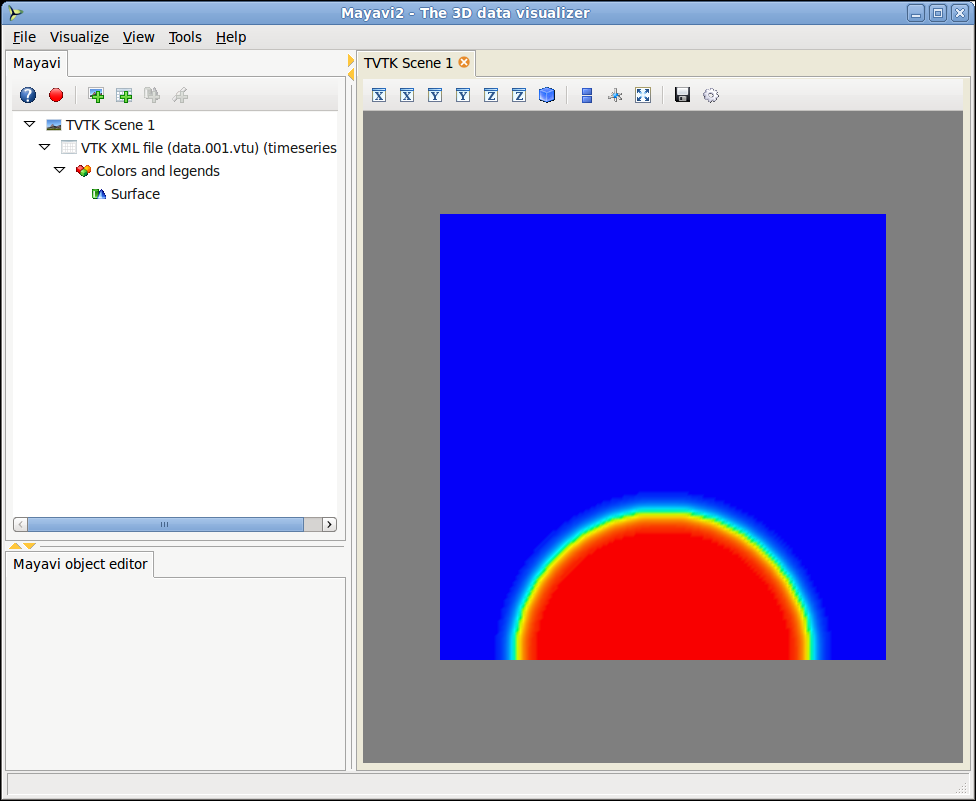
\includegraphics[width=4.in]{figures/ScreeshotMayavi2n1}}
\caption{Example 3b: \mayavi start up window}
\label{fig:mayavi window}
\end{figure}

\begin{figure}[ht]
\centerline{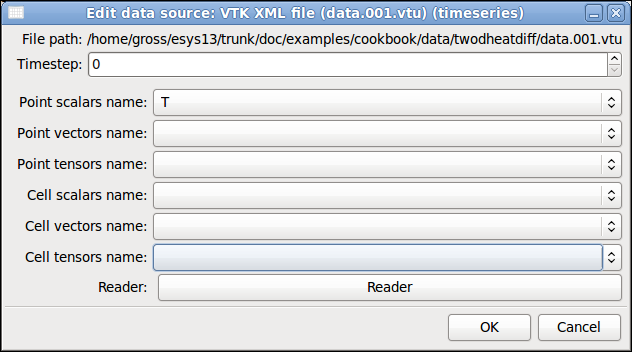
\includegraphics[width=4.in]{figures/ScreeshotMayavi2n2}}
\caption{Example 3b: \mayavi data control window}
\label{fig:mayavi window2}
\end{figure}
After you run the script you will find the 
result files \file{data.*.vtu} in the result directory \file{data/example03}.
Run the command
\begin{python}
>> mayavi2 -d data.001.vtu -m Surface &
\end{python}
from the result directory. \mayavi will start up a window similar to
\reffig{fig:mayavi window}.
The right hand side shows the temperature at the first time step. To show
the results at other time steps you can click at the item \texttt{VTK XML file
(data.001.vtu) (timeseries)}
at the top left hand side. This will bring up a new window similar to the window
shown in \reffig{fig:mayavi window2}. By clicking at the arrows in the top
right corner you can move forwards and backwards in time. 
You will also notice the text \textbf{T} next to the item \texttt{Point scalars
name}. The
name \textbf{T} corresponds to the keyword argument name \texttt{T} we have
used in the \verb|saveVTK| call. In this menu item you can select other results
you may have written to the output file for visualisation.

\textbf{For the advanced user}: Using the \modmpl to visualise spatially
distributed data is not MPI compatible. However, the \verb|saveVTK| function
can be used with MPI. In fact, the function collects the values of the sample
points spread across processor ranks into a single file.
For more details on writing scripts for parallel computing please consult the
\emph{user's guide}.




\chapter{Complex Geometries}
\label{CHAP HEAT 2}

%%%%%%%%%%%%%%%%%%%%%%%%%%%%%%%%%%%%%%%%%%%%%%%%%%%%%%%%
%
% Copyright (c) 2003-2010 by University of Queensland
% Earth Systems Science Computational Center (ESSCC)
% http://www.uq.edu.au/esscc
%
% Primary Business: Queensland, Australia
% Licensed under the Open Software License version 3.0
% http://www.opensource.org/licenses/osl-3.0.php
%
%%%%%%%%%%%%%%%%%%%%%%%%%%%%%%%%%%%%%%%%%%%%%%%%%%%%%%%%

\section{Steady-state Heat Refraction}
\label{STEADY-STATE HEAT REFRACTION}

In this chapter we will learn how to handle more complex geometries. 

Steady-state heat refraction will give us an opportunity to investigate some of the richer features that the \esc package has to offer. One of these is \pycad . The advantage of using \pycad is that it offers an easy method for developing and manipulating complex models. In conjunction with \gmsh we can generate finite element meshes that conform to our domain's shape providing accurate modeling of interfaces and boundaries. Another useful function of \pycad is that we can tag specific areas of our domain with labels as we construct them. These labels can then be used in \esc to define properties like material constants and source locations. 

We will introduce in two stages. First we will look at a very simple geometry. In fact,  we will solve 
the steady-state heat equation over a rectangular domain. This is not a very interesting problem but in a second
step we will extend our script by introducing an internal, curved interface.

\begin{figure}[ht]
\centerline{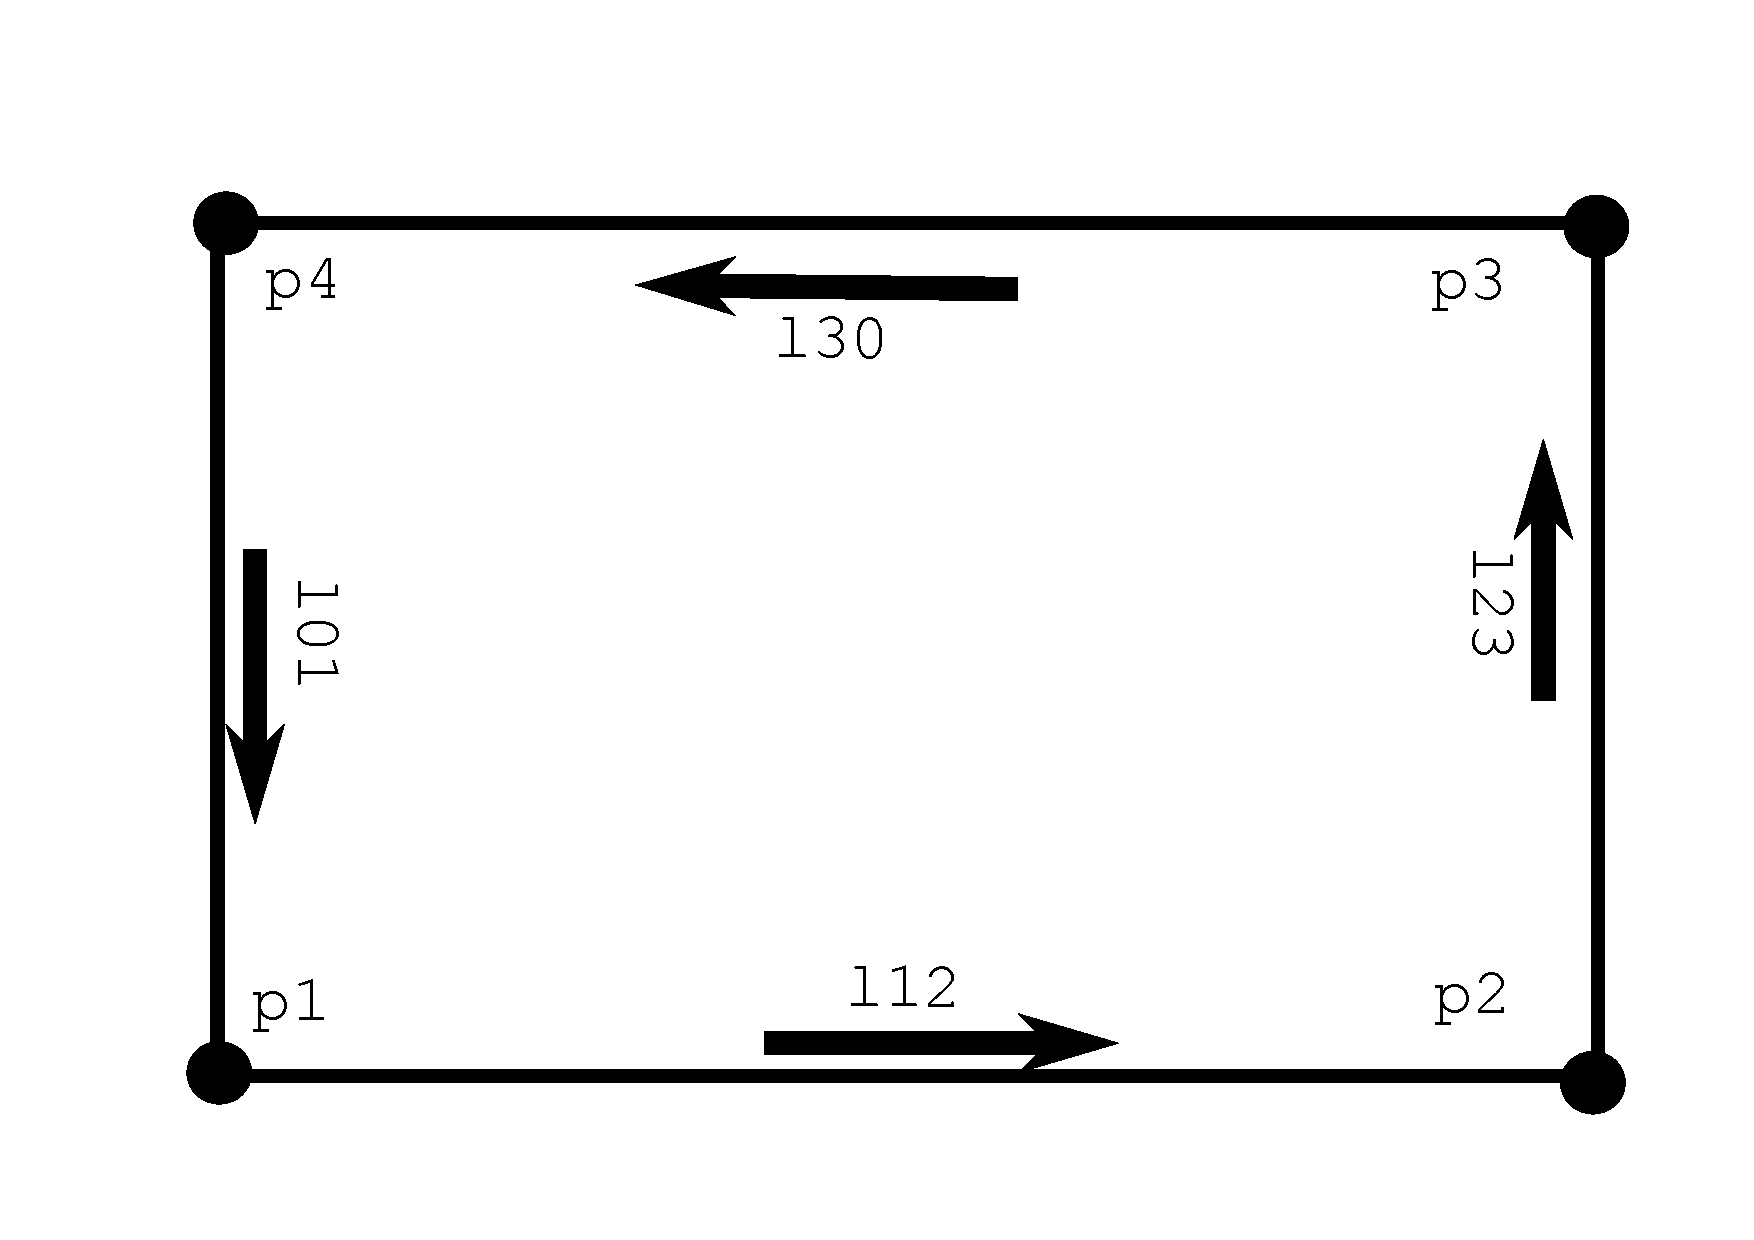
\includegraphics[width=4.in]{figures/pycadrec}}
\caption{Rectangular Domain for \pycad.}
\label{fig:pycad rec}
\end{figure}

\section{Example 4: Creating the model with \pycad}
\sslist{example04a.py}

We will modify the example in Chapter~\ref{CHAP HEAT 2a} in two ways: firstly we will look the steady state 
case with slightly modified boundary conditions and secondly we will use a more flexible tool 
to generate to generate the geometry. Lets look at the geometry first. 

We want to define a rectangular domain of width $5 km$ and depth $6 km$ below the surface of the Earth. Under the assumption of a known temperature at the surface, a known heat flux at the bottom and 
insulation to both sides we want to calculate the steady-state temperature distribution. 

In \pycad there are a few primary constructors that build upon each other to define domains and boundaries; 
the ones we will use are:
\begin{python}
from esys.pycad import *
Point() #Create a point in space.
Line() #Creates a line from a number of points.
CurveLoop() #Creates a closed loop from a number of lines.
PlaneSurface() #Creates a surface based on a CurveLoop
\end{python}
So to build-up our domain as shown in \reffig{fig:pycad rec} we first need to create
the corner points. From the corner points we build the four edges of the rectangle. The four edges
form then a closed loop which defines our domain as a surface.
We start by inputting the variables we need to construct the model.
\begin{python}
width=5000.0*m   #width of model
depth=-6000.0*m  #depth of model
\end{python} 
The variables are then used to construct the four corners of our domain, which from the origin has the dimensions of 5000 meters width and -6000 meters depth. This is done with the \verb Point()  function which accepts x, y and z coordinates. Our domain is in two dimensions so z should always be zero. 
\begin{python}
# Overall Domain
p0=Point(0.0,      0.0, 0.0)
p1=Point(0.0,    depth, 0.0)
p2=Point(width, depth, 0.0)
p3=Point(width,   0.0, 0.0)
\end{python}
Now lines are defined using our points. This forms a rectangle around our domain;
\begin{python}
l01=Line(p0, p1)
l12=Line(p1, p2)
l23=Line(p2, p3)
l30=Line(p3, p0)
\end{python}
Notice that lines have a direction. These lines form the basis for our domain boundary, which is a closed loop.
\begin{python}
c=CurveLoop(l01, l12, l23, l30)
\end{python}
Be careful to define the curved loop in an \textbf{anti-clockwise} manner otherwise the meshing algorithm may fail.
Finally we can define the domain as
\begin{python}
rec = PlaneSurface(c)
\end{python}
At this point the introduction of the curved loop seems to be unnecessary but this concept plays an important role 
if holes are introduced. 

Now we are ready to handover the domain \verb|rec| to a mesher which subdivides the domain into triangles (or tetrahedron in 3D). In our case we use \gmsh. We create 
an instance of the \verb|Design| class which will handle the interface to \gmsh: 
\begin{python}
from esys.pycad.gmsh import Design 
d=Design(dim=2, element_size=200*m)
\end{python}
The argument \verb|dim| defines the spatial dimension of the domain\footnote{If \texttt{dim}=3 the rectangle would be interpreted as a surface in the three dimensional space.}. The second argument \verb|element_size| defines element size which is the maximum length of a triangle edge in the mesh. The element size needs to be choose with care in order to avoid very large meshes if you don't want to. In our case with an element size of $200$m 
and a domain length of $6000$m we will end up with about $\frac{6000m}{200m}=30$ triangles in each spatial direction. So will end up with about $30 \times 30 = 900$ triangles which is a size that can be handled easily.
We can easily add our domain \verb|rec| to the \verb|Design|;
\begin{python}
d.addItem(rec)
\end{python}
We have the plan to set a heat flux on the bottom of the domain. One can use the masking technique to do this
but \pycad offers a more convenient technique called tagging. With this techniques items in the domain are
named using the \verb|PropertySet| class. We can then later use this name to set values secifically for
those sample points located on the named items. Here we name the bottom face of the 
domain where we will set the heat influx:
\begin{python}
ps=PropertySet("linebottom",l12))
d.addItem(ps)
\end{python}
Now we are ready to hand over the \verb|Design| to \FINLEY:
\begin{python}
from esys.finley import MakeDomain
domain=MakeDomain(d)
\end{python}
The \verb|domain| object can now be used in the same way like the return object of the \verb|Rectangle| 
object we have used previously to generate a mesh. It is common practice to separate the 
mesh generation from the PDE solution. The main reason for this is that mesh generation can be computationally very expensive in particular in 3D. So it is more efficient to generate the mesh once and write it to a file. The mesh
can then be read in every time a new simulation is run. \FINLEY supports this in the following 
way~\footnote{An alternative are the \texttt{dump} and \texttt{load} functions. They using a binary format and tend to be much smaller.}
\begin{python}
# write domain to an text file
domain.write("example04.fly")
\end{python}
and then for recovery in another script;
\begin{python}
# read domain from text file
from esys.finley import ReadMesh
domain =ReadMesh("example04.fly")
\end{python}

\begin{figure}[ht]
\centerline{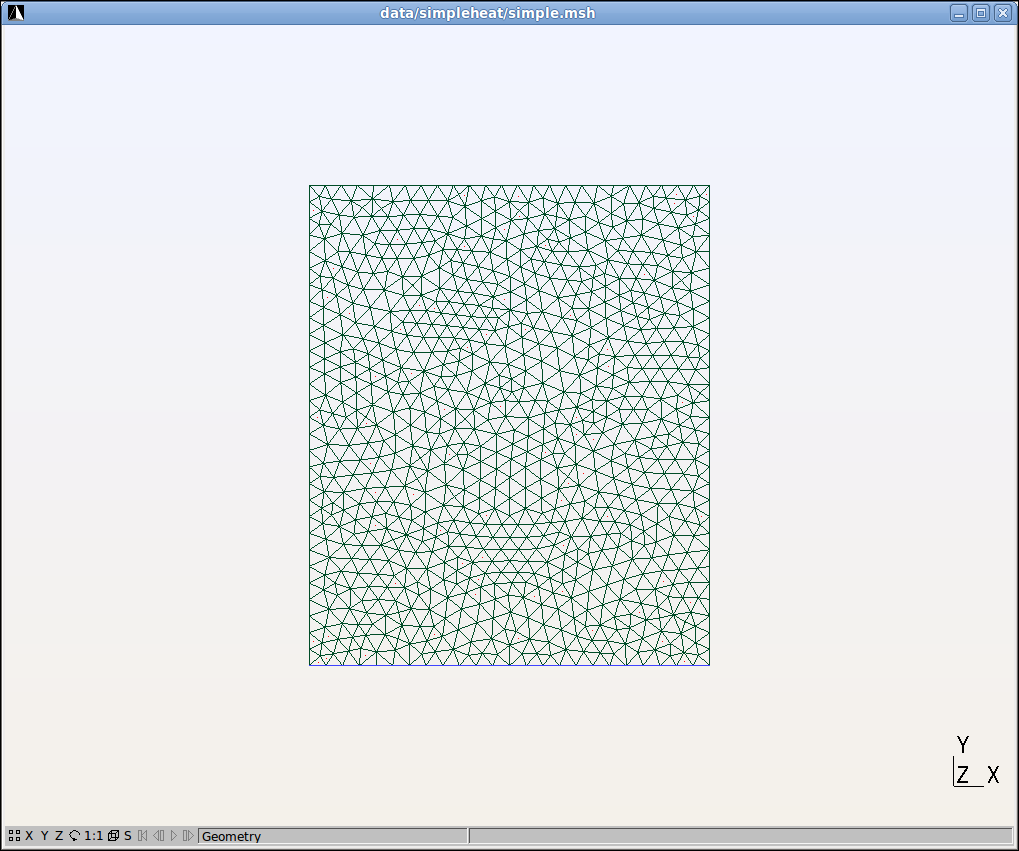
\includegraphics[width=4.in]{figures/simplemesh}}
\caption{Mesh over rectangular domain, see \reffig{fig:pycad rec}.}
\label{fig:pycad rec mesh}
\end{figure}

Before we discuss how we solve the PDE for the 
problem it is useful to present two additional options of the \verb|Design|. 
They allow the user accessing the script which is used to by \gmsh to generate the mesh as well as
the mesh as it has been generated by \gmsh. This is done by setting specific names for these files: 
\begin{python}
d.setScriptFileName("example04.geo")
d.setMeshFileName("example04.msh")
\end{python}
Usually the extension \texttt{geo} is used for the script file of the \gmsh geometry and
the extension \texttt{msh} for the mesh file. Normally these files are deleted after usage. 
Accessing these file can be helpful to debug the generation of more complex geometries. The geometry and the mesher can be visualise with \gmsh from the command line using
\begin{verbatim}
gmsh example04.geo  # show geometry
gmsh example04.msh  # show mesh
\end{verbatim}
The mesh is shown in \reffig{fig:pycad rec mesh}.
\begin{figure}[ht]
\centerline{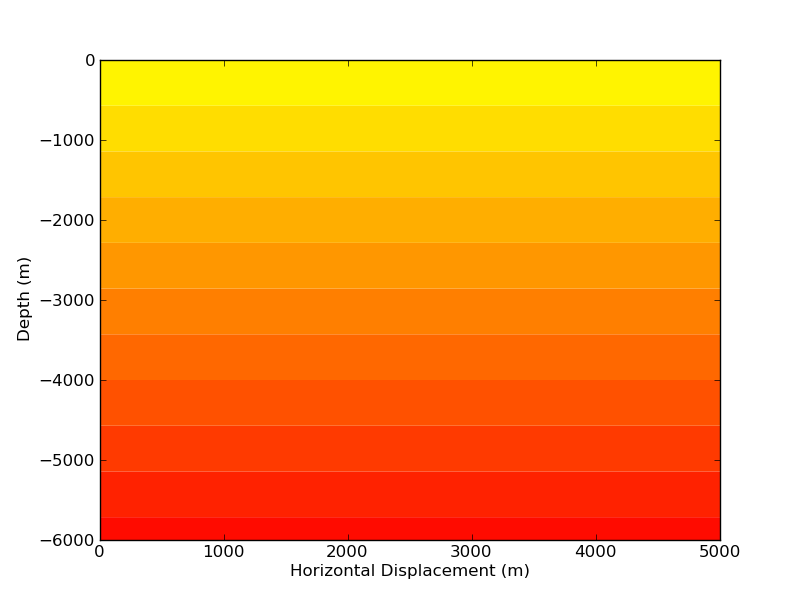
\includegraphics[width=4.in]{figures/simpleheat}}
\caption{Result of simple steady state heat problem.}
\label{fig:steady state heat}
\end{figure}


\section{The Steady-state Heat Equation}
\sslist{example04b.py, cblib}

Steady state is reached in the temperature is not changing in time. So to calculate the 
the steady state we set the time derivative term in \refEq{eqn:Tform nabla} to zero;
\begin{equation}\label{eqn:Tform nabla steady}
-\nabla \cdot \kappa \nabla T = q\hackscore H
\end{equation}
This PDE is easier then the PDE in \refEq{eqn:hdgenf2} we needed to solve in each time step. We can just drop
the \verb|D| term;
\begin{python}
mypde=LinearPDE(domain)
mypde.setValue(A=kappa*kronecker(model), Y=qH)
\end{python}
The temperature at the top face of the domain is known as \verb|Ttop| (=$20 C$). In \refSec{Sec:1DHDv0} we have 
already discussed how this constraint is added to the PDE:
\begin{python}
x=Solution(domain).getX()
mypde.setValue(q=whereZero(x[1]-sup(x[1])),r=Ttop)
\end{python}
Notice that we have use the \verb|sup| function to calculate the maximum $y$ coordinator of the relevant sample points.

In all cases so far we have assumed that the domain is insulated which translates 
into a zero normal flux $-n \cdot \kappa \nabla T$, see \refEq{eq:hom flux}. In the modeling
set-up of this chapter we want to set the normal heat flux at the bottom to \verb|qin| while we still
maintain insulation at the left and right face. Mathematically we can express this as the format
\begin{equation}
-n \cdot \kappa \nabla T = q\hackscore{S}
\label{eq:inhom flux}
\end{equation}
where $q\hackscore{S}$ is a function of its location on the boundary. Its value becomes zero
for locations on the left or right face of the domain while it has the value \verb|qin| at the bottom face.
Notice that the value of $q\hackscore{S}$ at the top face is not relevant as we prescribe the temperature here.
One could use the masking techniques we have already extensively used to define $q\hackscore{S}$ in \esc
but the tagging mechanism provides an alternative and in many cases more convenient way of defining piecewise 
constant functions such as $q\hackscore{S}$. You need to remember now that we
marked the bottom face with the name \verb|linebottom| when we defined the domain. 
We can use this now to create $q\hackscore{S}$;
\begin{python}
qS=Scalar(0,FunctionOnBoundary(domain))
qS.setTaggedValue("linebottom",qin)
\end{python}
In the first line \verb|qS| is defined as a scalar value over the sample points on the boundary of the domain. It is
initialized to zero for all sample points. In the second statement the values for those sample points which
on the line marked by \verb|linebottom| are set to \verb|qin|. 

The Neuman boundary condition assumed by \esc has in fact the form
\begin{equation}\label{NEUMAN 2b}
n\cdot A \cdot\nabla u = y 
\end{equation}
In comparison to the version in \refEq{NEUMAN 2} we have used so far the right hand side is now 
the new PDE coefficient $y$. As we have not specific $y$ in our previous examples \esc has assumed
the value zero for $y$. A comparison of \refEq{NEUMAN 2b} and \refEq{eq:inhom flux} reveals that one need to
choose $y=-q\hackscore{S}$;
\begin{python}
qS=Scalar(0,FunctionOnBoundary(domain))
qS.setTaggedValue("linebottom",qin)
mypde.setValue(y=-qS)
\end{python}
To plot the results we are using the \modmpl library as shown \refSec{Sec:2DHD plot}. For convenience
the interpolation of the temperature to a rectangular grid for contour plotting is made available
via the \verb|toRegGrid| function in the \verb|cblib| module. Your result should look similar to 
\reffig{fig:steady state heat}.

\begin{figure}[ht]
\centerline{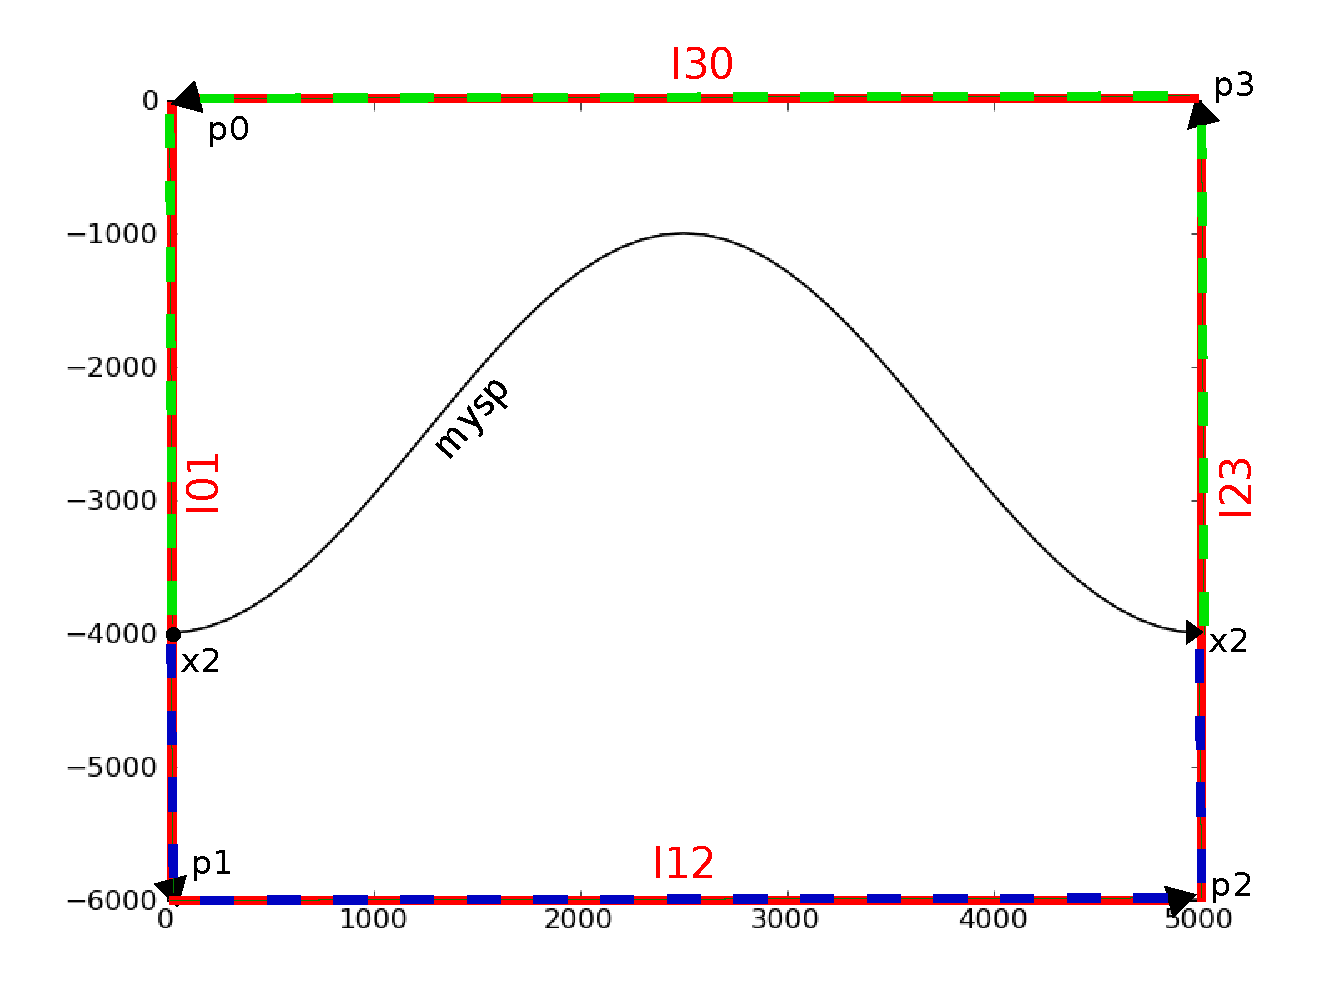
\includegraphics[width=4.in]{figures/anticlineheatrefraction}}
\caption{Heat refraction model with point and line labels.}
\label{fig:anticlinehrmodel}
\end{figure}

\begin{figure}[ht]
\centerline{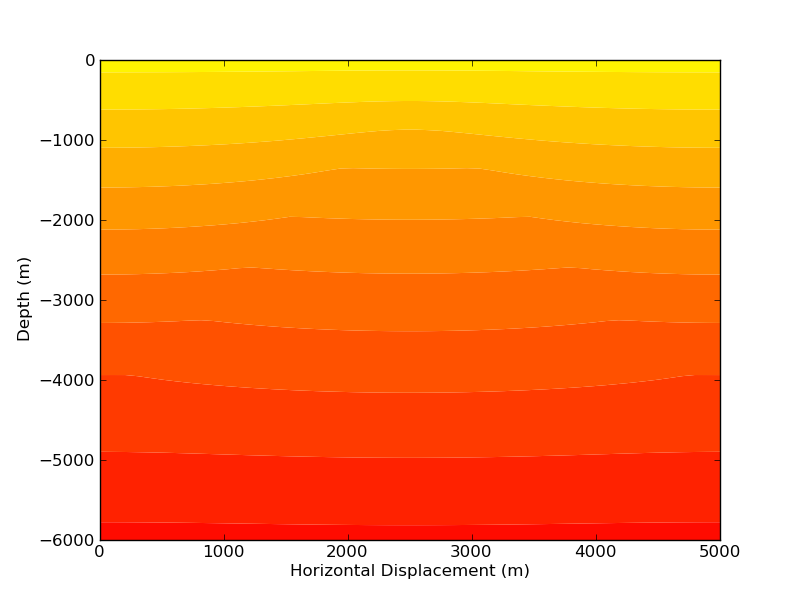
\includegraphics[width=4.in]{figures/heatrefraction}}
\caption{Temperature Distribution in the Heat Refraction Model.}
\label{fig:anticlinetemp}
\end{figure}

\section{A Heat Refraction model}
\sslist{heatrefraction_solver001.py and cblib.py}

Our heat refraction model will be a large anticlinal structure that is experiencing a constant temperature at the surface and a steady heat flux at it's base. Our aim is to show that the temperature flux across the surface is not linear from bottom to top but is in fact warped by the structure of the model and is heavily dependent upon the material properties and shape.


We will modify the example of the previous section by subdividing the block into two parts. The curve
separating the two blocks is given as a spline, see \reffig{fig:anticlinehrmodel}. The data points
used to define the curve may be measurement but for simplicity we assume here that there coordinates are
known in analytic form.

There are two modes available in our example. When \verb modal=1  this indicates to the script that we wish to model an anticline. Otherwise when \verb modal=-1  this will model a syncline. The modal operator simply changes the orientation of the boundary function so that it is either upwards or downwards curving. A \verb save_path  has also been defined so that we can easily separate our data from other examples and our scripts. 

It is now possible to start defining our domain and boundaries. 

The curve defining our clinal structure is located in approximately the middle of the domain and has a sinusoidal shape. We define the curve by generating points at discrete intervals; $51$ in this case, and then create a smooth curve through the points using the \verb Spline()  function.
\begin{python}
# Material Boundary
x=[ Point(i*dsp\
    ,-dep_sp+modal*orit*h_sp*cos(pi*i*dsp/dep_sp+pi))\
     for i in range(0,sspl)\
    ]
mysp = Spline(*tuple(x)) #*tuple() forces x to become a tuple
\end{python}
The start and end points of the spline can be returned to help define the material boundaries.
\begin{python}
x1=mysp.getStartPoint()
x2=mysp.getEndPoint()
\end{python}
The top block or material above the clinal/spline boundary is defined in a \textbf{anti-clockwise} manner by creating lines and then a closed loop. As we will be meshing the sub-domain we also need to assign it a planar surface. 
\begin{python}
# TOP BLOCK
tbl1=Line(p0,x1)
tbl2=mysp
tbl3=Line(x2,p3)
l30=Line(p3, p0)
tblockloop = CurveLoop(tbl1,tbl2,tbl3,l30)
tblock = PlaneSurface(tblockloop)
\end{python}
We must repeat the above for every other sub-domain. In this example there is only one other, the bottom block. The process is fairly similar to the top block but with a few differences. The spline points must be reversed by setting the spline as negative.
\begin{python}
bbl4=-mysp
\end{python}
This reverse spline option unfortunately does not work for the getLoopCoords command, however, the \modmpl polygon tool will accept clock-wise oriented points so we can define a new curve.
\begin{python}
#clockwise check
bblockloop=CurveLoop(mysp,Line(x2,p2),Line(p2,p1),Line(p1,x1))
\end{python}
The last few steps in creating the model take the previously defined domain and sub-domain points and generate a mesh that can be imported into \esc.
To initialise the mesh it first needs some design parameters. In this case we have 2 dimensions \verb dim  and a specified number of finite elements that need to be applied to the domain \verb element_size  . It then becomes a simple task of adding the sub-domains and flux boundaries to the design. Each element of our model can be given an identifier which makes it easier to define the sub-domain properties in the solution script. This is done using the \verb PropertySet()  function. The geometry and mesh are then saved so the \esc domain can be created.
\begin{python}
# Create a Design which can make the mesh
d=Design(dim=2, element_size=200)
# Add the sub-domains and flux boundaries.
d.addItems(PropertySet("top",tblock),PropertySet("bottom",bblock),\
                   PropertySet("linebottom",l12))
# Create the geometry, mesh and \esc domain
d.setScriptFileName(os.path.join(save_path,"heatrefraction.geo"))
d.setMeshFileName(os.path.join(save_path,"heatrefraction.msh"))
domain=MakeDomain(d,optimizeLabeling=True)
\end{python}
The creation of our domain and its mesh is complete.

With the mesh imported it is now possible to use our tagging property to set up our PDE coefficients. In this case $\kappa$ is set via the \verb setTaggedValue()  function which takes two arguments, the name of the tagged points and the value to assign to them. 
\begin{python}
# set up kappa (thermal conductivity across domain) using tags
kappa=Scalar(0,Function(domain))
kappa.setTaggedValue("top",2.0*W/m/K)
kappa.setTaggedValue("bottom",4.0*W/m/K)
\end{python}
No further changes are required to the PDE solution step, see \reffig{fig:anticlinetemp} for the result. 

\begin{figure}
\centering
    \subfigure[Temperature Depth Profile]{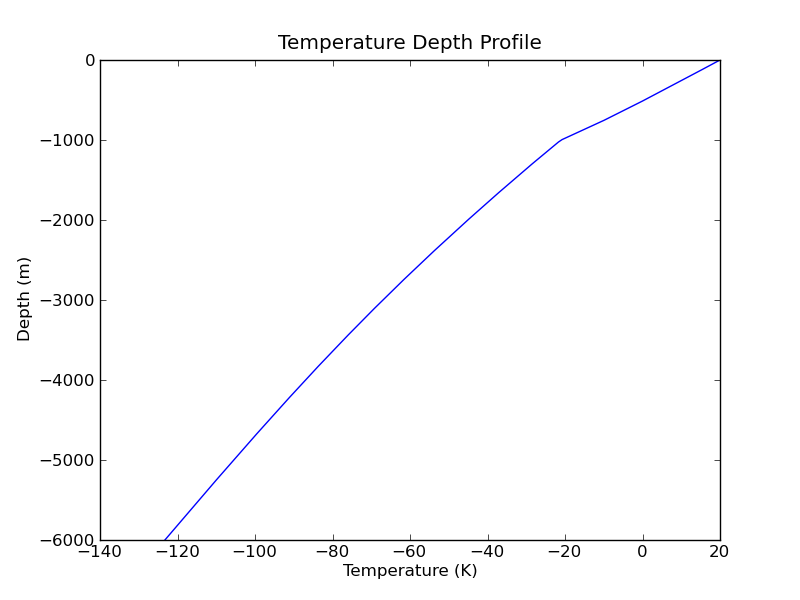
\includegraphics[width=3in]{figures/heatrefractiontdp.png}\label{fig:tdp}}
    \subfigure[Temperature Gradient Depth Profile]{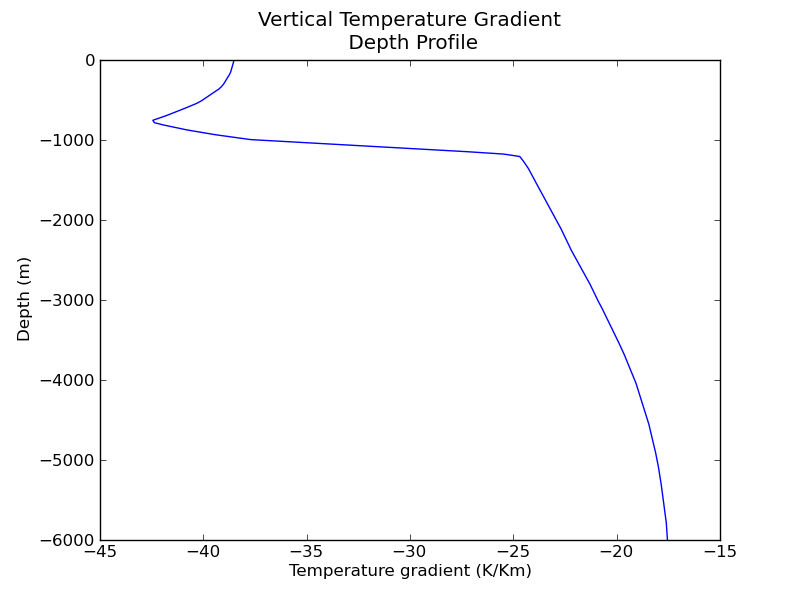
\includegraphics[width=3in]{figures/heatrefractiontgdp.png}\label{fig:tgdp}}
    \subfigure[Thermal Conductivity Profile]{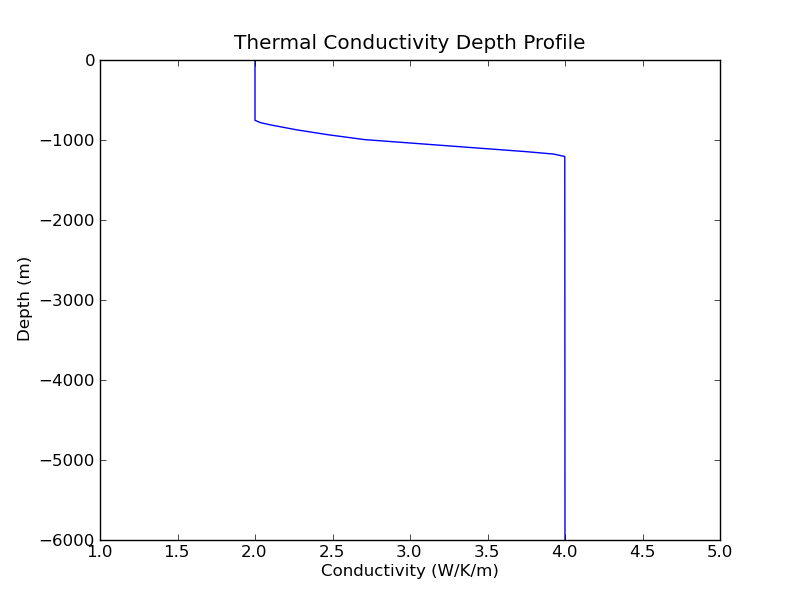
\includegraphics[width=3in]{figures/heatrefractiontcdp.png}\label{fig:tcdp}}
    \subfigure[Heat Flow Depth Profile]{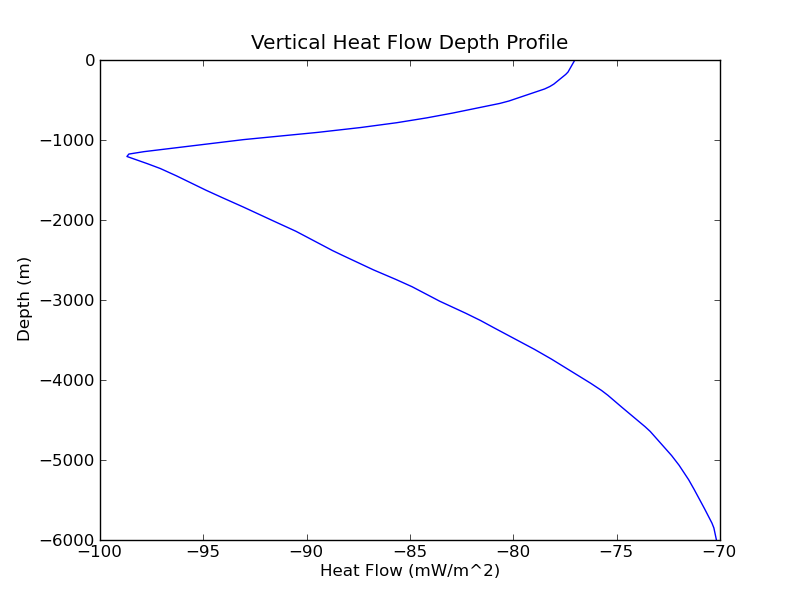
\includegraphics[width=3in]{figures/heatrefractionhf.png}\label{fig:hf}}
  \caption{Depth profiles down centre of model.}
  \label{figs:dps}
\end{figure}

\section{Line profiles of 2D data}
\sslist{heatrefraction_solver002.py and cblib.py}

We want to investigate the profile of the data of the last example. 
We are particularly interested in the deepth profile of the heat flux which is
the second component of $-\kappa \nabla T$. We will extend the script developed in the 
previous section to show how for instance vertical profile can be plotted.

The first important information is that \esc assumes that $-\kappa \nabla T$ is not smooth and
will in fact represent the values at numerical interpolation points. This assumption is reasonable as
the flux is the product of the piecewise constant function $\kappa$ and 
the gradient of the temperature $T$ which has a kink across the rock interface. 
Before plotting this function we need to smooth it using the 
\verb|Projector()| factory;
\begin{python}
from esys.escript.pdetools import Projector
proj=Projector(domain)
qu=proj(-kappa*grad(T))
\end{python}
The \verb|proj| object provides a mechanism to distribute values given at the numerical interpolation points
- in this case the heat flux - to the nodes of the FEM mesh. \verb|qu| has the same attached function space
like the temperature \verb|T|. The smoothed flux is interpolated 
to a regular $200\times 200$ grid;
\begin{python}
xiq,yiq,ziq = toRegGrid(qu[1],200,200)
\end{python}
using the \verb|toRegGrid| function from the cookbook library which we are already using for the contour plot.
At return \verb|ziq[j,i]| is the value of vertical heat flux at point 
(\verb|xiq[i]|,\verb|yiq[j]|). We can easily create deep profiles now by
plotting slices \verb|ziq[:,i]| over \verb|yiq|. The following script
creates a deep profile at $x_{0}=\frac{width}{2}$;
\begin{python}
cut=int(len(xiq)/2)
pl.plot(ziq[:,cut]*1000.,yiq)
pl.title("Vertical Heat Flow Depth Profile")
pl.xlabel("Heat Flow (mW/m^2)")
pl.ylabel("Depth (m)")
pl.savefig(os.path.join(save_path,"heatrefraction_hf.png"))
\end{python}
This process can be repeated for various variations of the solution. In this case we have temperature, temperature gradient, thermal conductivity and heat flow \reffig{figs:dps}.

\begin{figure}[ht]
\centerline{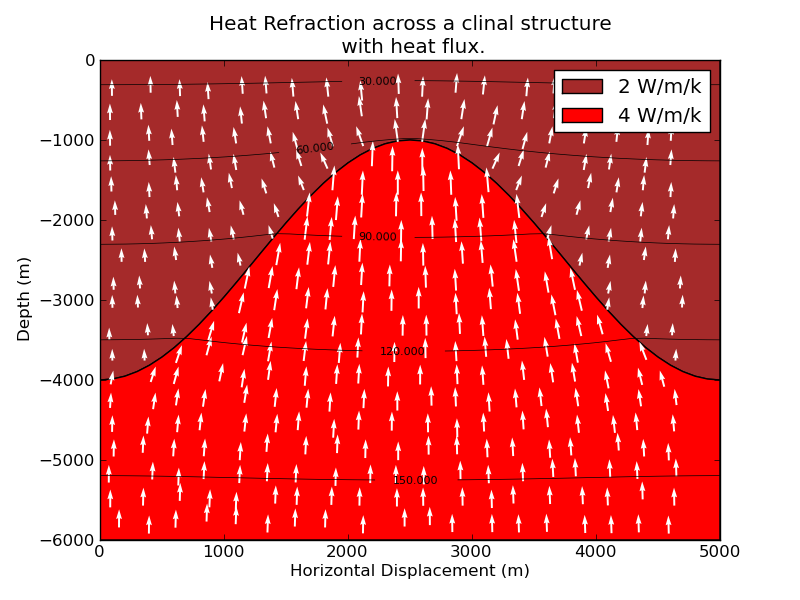
\includegraphics[width=5.in]{figures/heatrefractionflux}}
\caption{Heat refraction model with gradient indicated by vectors.}
\label{fig:hr001qumodel}
\end{figure}

\section{Arrow plots in \mpl}
\sslist{heatrefraction_solver003.py and cblib.py}
We would like to visualize the distribution of the flux $-\kappa \nabla T$ over the domain 
and produce a plot like shown in \reffig{fig:hr001qumodel}. 
The plot puts together three components. A contour plot of the temperature,
a colored representation of the two sub-domains where colour represents the thermal conductivity 
in the particular region and finally the arrows representing the direction of flux.

Contours have already been discussed in \refSec{Sec:2DHD plot}. To show sub-domains, 
we need to go back to \pycad data to get the points used to describe the boundary of the 
sub-domains. We have created the \verb|CurveLoop| class object 
\verb|tblockloop| to define the boundary of the upper sub-domain. 
We use the \verb|getPolygon()| method of \verb|CurveLoop| to get
access to the \verb|Point|s used top define the boundary. The statement
\begin{python}
[ p.getCoordinates() for p in tblockloop.getPolygon() ])
\end{python}
creates a list of the node coordinates of all the points in question. In order 
to simplify the selection of the $x$ and $y$ coordinates the list is converted 
into \modnumpy array. To add the area colored in brown to the plot we use; 
\begin{python}
import pylab as pl
import numarray as np
tpg=np.array([p.getCoordinates() for p in tblockloop.getPolygon() ])
pl.fill(tpg[:,0],tpg[:,1],'brown',label='2 W/m/k',zorder=-1000)
\end{python}
We can apply the same code to \verb|bblockloop| to a red area for this sub-domain to the block.

To plot vectors representing the flux orientation we use the 
\verb|quiver| function in \pylab. The function places vectors at locations in the domain.
For instance one can plot vectors at the locations of the sample points used by \esc 
to represent the flux \verb|-kappa*grad(T)|. As a vector is plotted at each sample point one typically ends
up with two many vectors. So one needs to select a subset of points:
First we create a coarse grid of points on a rectangular mesh, e.g. $20 \times 20$ points. Here we choose a grid of points which are located at the center of a \verb|nx| $\times$ \verb|ny| grid;
\begin{python}
dx = width/nx # x spacing
dy = depth/ny # y spacing
grid = [ ] # the grid points
for j in xrange(0,ny-1):
    for i in xrange(0,nx-1):
           grid.append([dx/2+dx*i,dy/2+dy*j])
\end{python}
With the \verb|Locator| \esc provides a mechanism to identify sample points that are closest 
to the the grid points we have selected and to get the data at these data points; 
\begin{python}
from esys.escript.pdetools import Locator
flux=-kappa*grad(T)
fluxLoc = Locator(flux.getFunctionSpace(),grid)
subflux= fluxLoc(flux) 
\end{python}
\verb|subflux| gives now a list of flux component at certain sample points. To get the 
list of the sample point coordinates one can use the \verb|getX()| method of the 
\verb|Locator|;
\begin{python}
subfluxloc = fluxLoc.getX()
\end{python}
To simplify the selection of $x$ and $y$ components it is convenient 
to transform \verb|subflux| and \verb|subfluxloc| to \numpy arrays
\verb|xflux|, \verb|flux|.
This function is implemented in the \verb|subsample| 
in the  \file{clib.py} file so we can use it in other examples. One can easily use this function 
to create a vector plot of the flux;
\begin{python}
from cblib import subsample
xflux, flux=subsample(-kappa*grad(T), nx=20, ny=20)
pl.quiver(xflux[:,0],xflux[:,1],flux[:,0],flux[:,1], angles='xy',color="white")
\end{python}
We add title and labels;
\begin{python}
pl.title("Heat Refraction across a clinal structure.")
pl.xlabel("Horizontal Displacement (m)")
pl.ylabel("Depth (m)")
pl.title("Heat Refraction across a clinal structure \n with gradient quivers.")
pl.savefig(os.path.join(saved_path,"heatrefractionflux.png"))
\end{python} 
to get the desired result, see \reffig{fig:hr001qumodel}.

\begin{figure}[ht]
\centerline{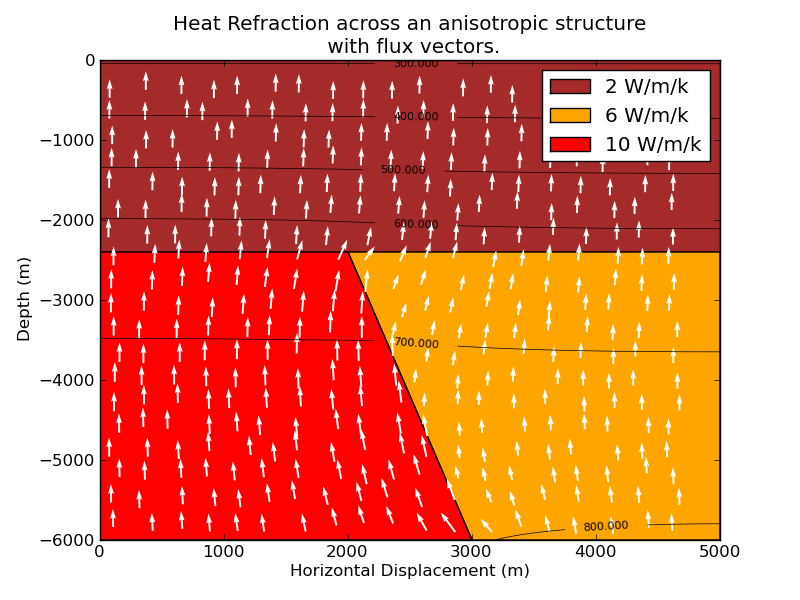
\includegraphics[width=4.in]{figures/heatrefraction2flux}}
\caption{Heat refraction model with three blocks and heat flux.}
\label{fig:hr002qumodel}
\end{figure}

\section{Fault and Overburden Model}
\sslist{heatrefraction2_solver.py and cblib.py}
A slightly more complicated model can be found in the examples \textit{heatrefraction2_solver.py} where three blocks are used within the model, see~\reffig{fig:hr002qumodel}. It is left to the reader to work through this example.




% Moving into 2D and 3D wave propagations in next chapters.
% not part of release 3.1
% \chapter{Seismic Wave Propagation}
% 
%%%%%%%%%%%%%%%%%%%%%%%%%%%%%%%%%%%%%%%%%%%%%%%%%%%%%%%%
%
% Copyright (c) 2003-2009 by University of Queensland
% Earth Systems Science Computational Center (ESSCC)
% http://www.uq.edu.au/esscc
%
% Primary Business: Queensland, Australia
% Licensed under the Open Software License version 3.0
% http://www.opensource.org/licenses/osl-3.0.php
%
%%%%%%%%%%%%%%%%%%%%%%%%%%%%%%%%%%%%%%%%%%%%%%%%%%%%%%%%

\section{Seismic Wave Propagation in Two Dimensions}
\editor{This chapter aims to expand the readers understanding of escript by modelling the wave equations.
Challenges will include a second order differential (multiple initial conditions). A new PDE to fit to the general form. Movement to a 3D problem (maybe)??? }

\verb|wavesolver2d.py|

Wave propagation in the earth can be described by the wave equation:
\begin{equation} \label{eqn:wav} \index{wave equation}
\rho \frac{\partial^{2}u\hackscore{i}}{\partial t^2} - \frac{\partial \sigma\hackscore{ij}}{\partial\hackscore{j}} = 0
\end{equation}
where $\sigma$ represents stress and is given by:
\begin{equation} \label{eqn:sigw}
 \sigma \hackscore{ij} = \lambda u\hackscore{k,k} \delta\hackscore{ij} + \mu ( u\hackscore{i,j} + u\hackscore{j,i})
\end{equation}
$\lambda$ and $\mu$ are the Lame Coefficients. Specifically $\mu$ is the bulk modulus. Equation \ref{eqn:wav} can be written with the Einstein summation convention as:
\begin{equation}
 \rho u\hackscore{i,tt} = \sigma\hackscore{ij,j}
\end{equation}
For this model we will specify the boundary conditions such that the normal of the stress from the boundary is zero.
\begin{eqnarray} \label{eqn:bdw}
\sigma \hackscore{ij}n\hackscore{j}=0
\end{eqnarray}
To solve this PDE we are going to write a more generic solution routine than we have in the previous chapters. There are a number of advantages to this approach. Firstly, by writing a subroutine that will solve a 2D wave propagation problem it reduces the amount of code duplication that may occur. When errors arrise one need only ammend the subroutine rather than all iterations of it that may have been created. This saves time and effort in the long run. 

To create the our subroutine we will need to import all our necessary libraries again. This is as for previous examples. Then we can define our script and the variables it will take. Our subroutine is located in \verb|/examples/cblib/wavesolver2d.py|  . The arguments of the subroutine are;
\begin{verbatim}
domain  : domain to solve over
h       : time step
tend    : end time
lam, mu : lames constants for domain
rho	: density of domain
U0	: magnitude of source
xc	: source location in domain (Vector)
savepath: where to output the data files
\end{verbatim}
There are a few differences between the wave equation and the heat diffusion problem of the previous chapter. While the nodes are defined the same way with the function \verb getX  and the PDE is still linear; one must consider the solution method. Without the line;
\begin{verbatim}
mypde.setSolverMethod(LinearPDE.LUMPING)
\end{verbatim}
the PDE would take a significant amount of time to solve. The \verb LUMPING  functionality implements an aggressive approximation for the $D$ coefficient matrix of the \esc linear PDE general form. While \verb LUMPING  introduces additional error to the solution it can significantly reduce the solution time. Care should be taken however, as this function can only be used when the $A$, $B$ and $C$ coefficients of the general form are zero. 

As the wave equation has a double time derivative, it is not sufficient to only stipulate the initial conditions for one time step. Two time steps must be specified so that the equation can be solved. For this example $u$ (\verb u ) and $u(t-1)$ (\verb u_m1 ) will be the same but if both of these condititions are known, they can be specified individually. It should be noted here that if multiple time steps are known at the begining of a model, they can be added to the simulation manually. The solver can then continue the model from the end of the known data. Alternatively, if the source motion is understood, its position can be corrected for each iteration to create a more accurate recreation of an event. 

The source in this example will induce a radially propagating wave. A small displacement will be applied to the medium about a singularity which we have called \verb xc  , this is the source location. We start by giving the source some spatial magnitude by defining a small radius about \verb xc  which is affected. The \verb src_radius  needs to cover a significant portion of grid nodes, otherwise the waves generated will suffer from dispersion due to an inadequate grid step size. If the source is small, the grid stepping must reflect the size of the source for more accurate results. Our radius will be;
\begin{verbatim}
 src_radius = 50
\end{verbatim}
Now that the extent of the source has been allocated it needs two more things; a direction and a magnitude. We can choose a direction based on the 360 degrees that exist in a full circle. If we take $\theta=0$ to be the x-axis and move counter clockwise then we can create a directional vector $U=[dx,dy]$  where $tan(\theta) = dy/dx$. It is also necessary to ensure that our directional vector of unit length such that $|U|=1$; which implies $\sqrt{dx^2+dy^2}=1$. By doing this we ensure that no accidental scaling is introduced to our source term. Here are three examples of different directions which satisfy the above conditions;
\begin{enumerate}
 \item Along the x-axis: $U=[dx=1,dy=0]$
 \item Along the y-axis: $U=[dx=0,dy=1]$
 \item At 45deg: $U=[dx=\frac{1}{\sqrt2},dy=\frac{1}{\sqrt2}]$
\end{enumerate}
There are limitations to specifying the source in this manner. Realistically we would not expect a 2D surface source to move form side to side as an isotropic source makes more sense. \editor{I am not sure here how to create an isotropic source function.}. In the 3D case things are not quite so bad. Normally we are interested in the p-waves that are directed dowwards and thus we need not have any x or y component in our source directionality. This still introduced assumptions and removes realistic wave motions both P and S from the model.
For our example we will use;
\begin{verbatim}
 dunit=numarray.array([1.,0.])
\end{verbatim}
Next we must define the values of our entire domain for the first and second time step. For the purposes of this example it is sufficient to have these two timesteps as equal. Setting the source is similar to earlier problems where we can use \esc functions to set specific areas of the domain to certain values. We must also smooth our sourse to its surrounds to prevent ?diffusion? errors. This is acheived by using a cosine taper. Our source terms then become;
\begin{verbatim}
 u=U0*(cos(length(x-xc)*3.1415/src_radius)+1)*\
              whereNegative(length(x-xc)-src_radius)*dunit
 u_m1=u
\end{verbatim}

It is often useful to know the values of PDE at certain locations in the model. To acheive this we are going to use a new generic function called \verb cbphones  which allows us to specify receiver locations to record the PDE values at those points. The function \verb cbphones as the arguments;
\begin{verbatim}
#	domain  : domain of model
#	U       : Current time state displacement solution.
#	phones  : Geophone Locations
#	dim     : model dimesions
#	savepath: where to output the data files local is default
\end{verbatim}
\editor{not generic as of yet but may move to make cbphones and the phones positioning a serious part of wavesolver 2d}
We have chosen to have three receivers and they are called using;
\begin{verbatim}
u_pot = cbphones(domain,u,[[0,500],[250,500],[400,500]],2)
\end{verbatim}
This places the receivers on the surface at the source location and two locations further along the top of the model. The output \verb u_pot  can then be split and saved to file using the following command;
\begin{verbatim}
u_pc_data=open(os.path.join(savepath,'U_pc.out'),'w')
u_pc_data.write("%f %f %f %f %f %f %f\n"%(t,u_pc_x1,u_pc_y1,u_pc_x2,u_pc_y2,u_pc_x3,u_pc_y3))
\end{verbatim}
Convieniently this saves the time, x direction displacement and y direction displacement values for these locations. Now that the initial conditions have been defined we can tackle the task of solving the wave equation for the number of required time steps. To do this we require a while loop and form of the wave equation which fits our general linear PDE form. We start with the form of the equation for stress \ref{eqn:sigw}. We can define the kronecker matrix using the domain and take the derivative of \verb u  via the function \verb|grad(u)|  . As $\lambda$ and $\mu$ are constants we can now define $\sigma$;
\begin{verbatim}
g=grad(u)
stress=lam*trace(g)*kmat+mu*(g+transpose(g))
\end{verbatim}
Solving for the double time derivative of u on the LHS of \ref{eqn:wav} required us to use the centred difference forumlua which returns;
\begin{equation}
u^n = 2u^{n-1}-u^{n-2}+h^2 \biggl(\frac{\partial ^2 u}{\partial t^2}\biggr)^n
\end{equation}
Substituting for the double time derivative we see;
\begin{equation}
\rho u^n = 2\rho u^{n-1}- \rho u^{n-2}+h^2 \sigma \hackscore{ij,j} ^n
\end{equation}
This fits the general form $Du=-X \hackscore{j,j} + Y$ where $D=rho$; $Y=2\rho u^{n-1}- \rho u^{n-2}$ and $X=-h^2 \sigma \hackscore{ij,j} ^n$. \verb D does not vary between time steps can be defined before our iteration loop via;
\begin{verbatim}
mypde.setValue(D=kmat*rho)
\end{verbatim}
The values for \verb u  must be refreshed after each iteration and are thus defined within our while loop via;
\begin{verbatim}
mypde.setValue(X=-stress*(h*h),Y=(rho*2*u-rho*u_m1))
\end{verbatim}
With each iteration we update \verb u  and migrate our answers into the correct variables. The iterative values must also be updated as well as the response from our receiver locations. All this is acheived via;
\begin{verbatim}
u_p1 = mypde.getSolution()
u_m1=u
u=u_p1
t+=h
n+=1
u_pot = cbphones(domain,u,[[125.,250.],[250.,250.],[250.,375.]],2)
# save displacements at point source to file for t > 0
u_pc_data.write("%f %f %f %f %f %f %f\n"%(t,u_pc_x1,u_pc_y1,u_pc_x2,u_pc_y2,u_pc_x3,u_pc_y3))
\end{verbatim}
With an appropriate file saving output we now have a working generic solver for our 2D wave equation problem. We have also included our two new generic programs in the \verb cblib  library so they can be more simply imported along with their own dependancies to our test script.

Writing a test program will allow us to more easily pass the variables required to the solver to generate an output solution. Our testing code described in this section can be found in \fileex{wavesolver2d001.py}. In a similar manner to the previous chapter the first step to creating our script is to import the necessary modules and functions including our new library file. Following this the PDE and control variables must be defined. This includes the domain dimensions and type, the time scale and the time step. To ensure stability the time step can be calcuated such that it satisfies the Courant stability criteria \editor{MORE HERE ONCE METHOD FINALISED}. Considering the complexity of the computational solution to the wave equation it is proudant to consider how many steps will need to be solved. Our test script thus includes an acknowledgement clause;
\begin{verbatim}
#Check to make sure number of time steps is not too large.
print "Time step size= ",h, "Expected number of outputs= ",tend/h
proceeder = raw_input("Is this ok?(y/n)")
#Exit if user thinks too many outputs.
if proceeder == "n":
sys.exit()
\end{verbatim}
This requires that the user knows the number of itterations that will be required to solve the model for the time period \verb 0  to \verb tend . The command \verb sys.exit()  is used here to halt the script if the input to preceeder is \verb n  and thus prevent a forced crash of the script should its projected solve time be too large.



%%%%%%%%%%%%%%%%%%%%%%%%%%%%%%%%%%%%%%%%%%%%%%%%%%%%%%%%%%%%%%%%%%%%%%%%%%%%%%
% Copyright (c) 2003-2012 by University of Queensland
% http://www.uq.edu.au
%
% Primary Business: Queensland, Australia
% Licensed under the Open Software License version 3.0
% http://www.opensource.org/licenses/osl-3.0.php
%
% Development until 2012 by Earth Systems Science Computational Center (ESSCC)
% Development since 2012 by School of Earth Sciences
%
%%%%%%%%%%%%%%%%%%%%%%%%%%%%%%%%%%%%%%%%%%%%%%%%%%%%%%%%%%%%%%%%%%%%%%%%%%%%%%

\chapter{The Einstein Summation Convention}

The Einstein Summation Convention (ESC) is a notational convention that is prefered by the \esc developers. It is a condensed and practical way to deal with multi-dimensional and convoluted PDEs. By suppressing the need to write out the many terms of each problem it is possible to increase efficiency and reduce the number of errors created through poor working. According to the convention, when an index variable appears twice in a single term, it implies that we are summing over all of its possible values.
So we have;
\begin{equation}
a_{1}\frac{\partial^2 f}{\partial x_{1}^2} + a_{2}\frac{\partial^2 f}{\partial x_{2}^2} = a_{i}\frac{\partial^2 f}{\partial x_{i}^2}
\end{equation}

For a scalar function $f(x_{1},x_{2},..x_{i})$ and a vector $\mathbf{u}(u_{1},u_{2},..u_{i})$ with $u_{i}(x_{1},x_{2},..x_{i})$, we have the following notation:
\begin{equation}
\mathbf{u}=\sum_{i}u_{i}e^i = u_{i}e^i
\end{equation}
\begin{equation}
\mathbf{grad}(f) = \mathbf{\nabla}(f) = \sum_{i}\frac{\partial f}{\partial x_{i}}e^i = (\partial_{i} f)e^i = f_{,i}e^i
\end{equation}
\begin{equation}
div(\mathbf{u}) = \mathbf{\nabla}.\mathbf{u} = \sum_{i}\frac{\partial u_{i}}{\partial x_{i}} = \partial_{i} u_{i} = u_{i,i}
\end{equation}
\begin{equation}
div(\mathbf{grad}(f)) = \nabla^2 f = \Delta f = \sum_{i}\frac{\partial^2 f}{\partial x_{i}^2} = f_{,ii}
\end{equation}

\end{document}
